\documentclass[11pt,letterpaper]{article}
\usepackage[T1]{fontenc}
\usepackage[utf8]{inputenc}
\usepackage{lmodern,microtype}
\usepackage[margin=0.85in,headheight=15pt,headsep=18pt,footskip=25pt]{geometry}
\usepackage{amsmath,amssymb,mathtools}
\usepackage{booktabs,longtable,array,tabularx}
\usepackage{xcolor,graphicx,float}
\usepackage[font=small,labelfont={bf,sf},labelsep=period]{caption}
\usepackage{xurl}
\usepackage{tikz}
\usetikzlibrary{arrows.meta,positioning,fit,calc,shapes.geometric,decorations.pathmorphing}
\usepackage{enumitem,needspace}
\usepackage{titlesec,fancyhdr,lastpage}
\usepackage{listings}
\usepackage[numbers,sort&compress]{natbib}
\usepackage[colorlinks=true,linkcolor=teal,citecolor=teal,urlcolor=teal]{hyperref}
\definecolor{ink}{HTML}{19333C}
\definecolor{teal}{HTML}{176D76}
\definecolor{muted}{HTML}{51616B}
\definecolor{pale}{HTML}{EEF4F5}
\definecolor{accent}{HTML}{C26A2E}
\definecolor{warnpale}{HTML}{FBF1EA}
\pagestyle{fancy}
\fancyhf{}
\fancyhead[L]{\footnotesize\sffamily\color{muted}RaoRocketSim / MOC solver extensions plan}
\fancyhead[R]{\footnotesize\sffamily\color{muted}21 November 2026}
\fancyfoot[R]{\footnotesize\sffamily\color{muted}\thepage\ / \pageref*{LastPage}}
\renewcommand{\headrulewidth}{0.3pt}
\titleformat{\section}{\Large\sffamily\bfseries\color{ink}}{\thesection}{0.7em}{}
\titleformat{\subsection}{\large\sffamily\bfseries\color{teal}}{\thesubsection}{0.6em}{}
\titleformat{\subsubsection}{\normalsize\sffamily\bfseries\color{ink}}{\thesubsubsection}{0.6em}{}
\setlength{\parindent}{0pt}
\setlength{\parskip}{6pt}
\setlength{\emergencystretch}{2em}
\renewcommand{\arraystretch}{1.15}
\setlist{itemsep=3pt,topsep=4pt,leftmargin=1.6em}
\newcolumntype{P}[1]{>{\raggedright\arraybackslash}p{#1}}
\newcommand{\code}[1]{{\small\path{#1}}}
\newcommand{\dd}{\mathrm{d}}
\newcommand{\Rt}{R_t}
\newcommand{\decision}[1]{\par\medskip\noindent\begingroup\setlength{\fboxsep}{9pt}\colorbox{pale}{\parbox{\dimexpr\linewidth-18pt\relax}{#1}}\endgroup\par\medskip}
\newcommand{\caution}[1]{\par\medskip\noindent\begingroup\setlength{\fboxsep}{9pt}\colorbox{warnpale}{\parbox{\dimexpr\linewidth-18pt\relax}{\sffamily\bfseries\color{accent}Caution. \normalfont\rmfamily\color{black}#1}}\endgroup\par\medskip}
\newcommand{\buildfig}[4]{\begin{figure}[htbp]\centering\includegraphics[width=#3\linewidth,keepaspectratio]{#1}\caption{#2}\label{#4}\end{figure}}
\lstset{basicstyle=\ttfamily\footnotesize,breaklines=true,columns=fullflexible,keepspaces=true,showstringspaces=false,backgroundcolor=\color{pale},frame=none,xleftmargin=6pt,xrightmargin=6pt}
\numberwithin{equation}{section}

\hypersetup{pdftitle={MOC Solver Extensions},pdfsubject={Variable gas, shock fitting, viscous interaction and a differentiable forward net: plan and evidence}}
\usepackage{multicol}
\renewcommand{\bibfont}{\scriptsize}
\setlength{\bibsep}{0pt}
\setlength{\parskip}{3.5pt plus 1pt}
\setlist{itemsep=1pt,topsep=2pt,parsep=0pt,partopsep=0pt}
\titlespacing*{\section}{0pt}{11pt plus 2pt}{4pt}
\titlespacing*{\subsection}{0pt}{8pt plus 2pt}{3pt}
\setcounter{tocdepth}{1}
\newcounter{ltplain}
\renewcommand{\LTcaptype}{ltplain}
\newcommand{\keep}[1]{\par\needspace{#1\baselineskip}}
\begin{document}
\thispagestyle{empty}
{\huge\sffamily\bfseries\color{ink}MOC Solver Extensions\par}
\vspace{0.15cm}
{\large\sffamily\color{teal}Variable gas, shock fitting, viscous interaction and a differentiable forward net\par}
\vspace{0.15cm}
{\small RaoRocketSim / LREKit, subsystem S06 \hfill 21 November 2026\par}
\vspace{0.25cm}
\textbf{Purpose.} This plan extends and supersedes the draft roadmap
\emph{From MOC Verification to an Engine Solver Suite} (same date), revising its
milestone graph with page-checked literature and fourteen experiments plus follow-ups.

\textbf{Principal findings.}
\begin{itemize}
\item \textbf{Start line.} The third-order Kliegel--Levine (KL) start line carries a
sign error in one axisymmetric term, confirmed by three independent checks; the
production coefficients were not changed. A \emph{diagnostic} forward replay of the
accepted Nozzle-B wall, which was optimised with the uncorrected series, changes $C_F$
by $-1.22$\,\% with the corrected start line (307 times the t19 refinement band),
mostly through a $-1.25$\,\% change in mass flow. This is not a corrected design: the
corrected-series re-solve has not been run or approved (D10).
\item \textbf{Variable gas.} A thermodynamically consistent variable-gas MOC can keep
the existing unit processes: along one isentrope the turning function, Mach angle
and state are one-dimensional tables. In a manufactured test, a local $\gamma(T)$
in the constant-$\gamma$ Prandtl--Meyer function gives 7.3--8.9\,deg errors over
$M=1.05$--4, and a fixed chamber, throat or exit $\gamma$ gives 3.95--13.10\,deg (E03).
\item \textbf{Forward net.} A diagnostic exit-limited harness of the forward net
reproduces the BVP to $|\Delta C_F|/C_F=8.7\times10^{-6}$ (code-to-code, shared KL
start line). The production march stops at a fold outside the nozzle (E07); folds at
weak coalescences still block shock fitting and viscous coupling.
\item \textbf{LEA/TOP.} The two LEA/TOP length failures come from an undeclared split
between bell-length conventions. The repository's LEA case also uses a $0.382R_t$
throat arc where the source shows $0.5y_t$, and the source's $15.0r_t$ is most likely
$x_E-x_N$ (inferred), so the $15\pm0.02$ check was circular.
\item \textbf{Optimiser.} The engine optimiser closes thrust with a fixed efficiency on a
one-dimensional $C_F$. For Nozzle-B the MOC value is $0.9672$ of it with the production
start line ($C_D=1.0075$) and about $0.955$ in the corrected-start-line replay.
\end{itemize}
\textbf{Evidence classes.} \emph{Numerical verification}: an exact solution, a limit,
or code-to-code agreement between two repository algorithms on the same model.
\emph{Benchmark agreement}: agreement with published or digitised data, or with an
independent external code such as CFD. \emph{Physical validation}: agreement with
matched measurements of the physical system; this plan claims none.

Every new capability except the C0 result contract (typing and refusal of invalid
results) is opt-in; promotion to a default (D0) needs a user decision. No default,
tolerance, gate or coefficient was changed.

\vspace{0.3em}
\section*{\contentsname}
\makeatletter
{\footnotesize\setlength{\parskip}{0pt}\renewcommand{\addvspace}[1]{\vspace{0.5pt}}%
\setlength{\columnsep}{18pt}\begin{multicols}{2}\@starttoc{toc}\end{multicols}}
\makeatother
\section{Scope and terms}
\label{sec:scope}
The plan covers four primary gaps: G1, variable-gas thermodynamics; G2, shock fitting;
G3, viscous interaction and separation; and G4, a general differentiable forward-wall
net. It also covers the items the MOC audit logbook left open: the transonic start
line (MOC-08/09), the exact-axis limit (MOC-14), an independent reference and accuracy
envelope (MOC-15), the Young source-term discrepancy, the LEA/TOP length failures and
the optimiser architecture (ARCH). Each gap section gives equations with page sources,
compares approaches, chooses one and lists milestones with three acceptance columns;
Section~\ref{sec:experiments} reports the experiments.

\begingroup\footnotesize
\setlength{\parskip}{1.5pt}\setlength{\columnsep}{14pt}
\begin{multicols}{2}\raggedright
\textbf{Flow and geometry.}
\begin{itemize}
\item \textbf{Q1D:} quasi-one-dimensional isentropic relations, which the engine
optimiser (MDO) uses to close thrust and throat size.
\item \textbf{TOP/B\'ezier:} the default bell, a $0.382R_t$ throat arc ending at the
inflection point N at $\theta_N$, then a quadratic B\'ezier to the exit E at
$\theta_E$, with angles from the SP-125 chart.
\item \textbf{LEA:} the LEA\_TOP benchmark case of Schomberg et al.\ \cite{schomberg2019}.
\item \textbf{Nozzle-B:} Rao's example, with $\gamma=1.23$, $\epsilon=4.973$ and length
$2.94R_t$ \cite[PDF pp.~2--5, printed pp.~378--381]{rao1958}. Rao used a $0.45R_t$
arc and a Sauer start; the repository variant uses $R_u=1.5R_t$, $R_d=0.382R_t$ and
a KL start line.
\end{itemize}

\textbf{Characteristic net.}
\begin{itemize}
\item \textbf{RRC, LRC:} right-running ($C^-$) and left-running ($C^+$)
characteristics. The forward net marches RRC rows from the wall to the axis.
\item \textbf{Kernel, B, BD:} the expansion region between the start line and BD, the
last RRC leaving the end B of the throat arc.
\item \textbf{Raw and special rows:} a raw kernel row places its wall point where a
$C^+$ meets the arc; a special row inserts one at a limited turning step.
\item \textbf{Kernel capacity:} the maximum number of kernel rows.
\item \textbf{BDE, BVP:} Rao's inverse construction, a control surface DE (a $C^+$ from
D on BD to the exit lip E) with the wall built backward, solved as a boundary-value
problem.
\item \textbf{D/E attachment:} the opt-in exact elimination of the D state and of E
from the BVP unknowns.
\item \textbf{Seed controls:} the kernel-angle search that seeds the BVP.
\item \textbf{Fold:} a reversed characteristic cell, i.e.\ same-family characteristics
crossing; the march stops.
\end{itemize}

\textbf{Start line.}
\begin{itemize}
\item \textbf{Start line, KL:} transonic initial data from the Kliegel--Levine
third-order series in $1/(1+R_c/R_t)$.
\item \textbf{$M_{\min}$ push:} moving a start-line point downstream until it reaches
$M\ge1.05$.
\item \textbf{Spacelike margin:} the angle between the start line and the nearest
local characteristic.
\item \textbf{KL-V0 to KL-V3:} the start-line variants of Section~\ref{sec:kl}.
\item \textbf{D-K0-BVP:} the deferred corrected-start-line Nozzle-B re-solve (D10).
\end{itemize}

\textbf{Experiments and benchmarks.}
\begin{itemize}
\item \textbf{t19 pair, band:} the accepted 32/48 versus 48/64 Nozzle-B refinement
pair (logbook Iteration 19) and its differences.
\item \textbf{Gates:} the logbook's eleven physical and topology checks of a BVP
solution, such as $C^\pm$ compatibility, no crossings, wall tangency, the axis and
seams, and mass closure.
\item \textbf{Field coverage:} the fraction of one mesh's nodes inside the other's
hull.
\item \textbf{t01:} the logbook Iteration-01 fold runs on the $\epsilon=10$, 80\,\% TOP
bell.
\item \textbf{$J_1$--$J_3$:} the E12 outputs, namely the BD mass flow, the Mach number
at B and the axial station of the BD axis point.
\end{itemize}

\textbf{Tools and acronyms.}
\begin{itemize}
\item \textbf{TDK:} NASA's Two-Dimensional Kinetics nozzle program \cite{nickerson1985}.
\item \textbf{BLM:} TDK's boundary-layer module.
\item \textbf{$\eta_{\mathrm{DER}}$:} TDK's empirical efficiency factor in delivered
$I_{sp}$.
\item \textbf{FSS, RSS:} free and restricted shock separation.
\item \textbf{NPR:} the nozzle pressure ratio $p_0/p_a$.
\item \textbf{GCI:} the grid convergence index \cite{celik2008}.
\end{itemize}
\end{multicols}
\endgroup

\section{Current state from the MOC logbook}
\label{sec:current-state}
The logbook (Repository Guide, Chapter 15) closes with one accepted configuration:
Nozzle-B, inviscid and constant-$\gamma$, solved as a BVP with exact D/E attachment,
an explicit kernel capacity and accurate seed controls.
Both levels pass the eleven gates. The 32/48 to 48/64 comparison passes the unchanged
policy: Mach difference 0.00080366, flow-angle difference $0.0228912^\circ$ (limit
$0.05^\circ$), field coverage 0.950270. $C_F=1.57955$ is 0.212\,\% below Rao's 1.5829,
with different throat and start-line models. The pair took 1{,}497.5\,s. This is numerical verification of one configuration only.

The audit's 26 findings were 4 correct, 9 incorrect (all repaired), 6 incomplete,
3 uncertain and 4 missing. It left open MOC-08/09 (KL table and normalisation), MOC-14 (axis limit), MOC-15
(independent reference), MOC-16 (the extensions) and two LEA/TOP failures
($L/R_t=15.0448$ against $15\pm0.02$). Table~\ref{tab:new-rows} gives their status now, with five proposed new rows. The
optimiser closes thrust with a Q1D model before it requests geometry
(Section~\ref{sec:geometry-arch}).

\begingroup\footnotesize\renewcommand{\LTcaptype}{table}
\begin{longtable}{@{}P{0.09\linewidth}P{0.50\linewidth}P{0.35\linewidth}@{}}
\caption{Open and proposed traceability rows.}\label{tab:new-rows}\\
\toprule\textbf{ID} & \textbf{Finding} & \textbf{Status / action}\\\midrule
\endfirsthead
\toprule\textbf{ID} & \textbf{Finding} & \textbf{Status / action}\\\midrule
\endhead
MOC-08/09 & KL axisymmetric $v_3$ $zy^3$ sign wrong; four planar defects; $\sqrt{U^2+V^2}$ is $M^*$ & Confirmed; production unchanged; opt-in K0b\\
MOC-14 & Exact-axis source limit & Proposed: no active defect on the tested paths (E05, E06); the BVP's \code{_source_axisym} and JAX mirrors untested (X0 test before closing)\\
MOC-15 & Independent reference; accuracy envelope & Oracle exists; E05 FAIL as pre-registered (lip row). Post hoc: interior order 1.59--1.76, functionals $\approx2$ ($15^\circ$, E05b). CFD pending D1\\
MOC-27 & Near-axis closure: the exit-lip special row puts a point at 0.18--0.54 of the normal spacing (E05); at $n=64$ the sign-only (KL-V1) and $M^*$-only (KL-V2) start lines fail near the axis, KL-V3 does not (E09); a $\theta\ge0$ clamp switches inside $\theta_B$ windows (E12) & Open (N0, K0a, N2); the lip row does not contaminate exit-plane functionals (E05b)\\
MOC-28 & The forward net audits whole RRCs to the axis, so a fold outside the nozzle ends the replay (E07) & Fix verified in a diagnostic harness (E07b); production opt-in in N0\\
MOC-29 & The production start line passes more than the ideal throat mass flow ($C_D=1.0075$) & Open (K0); KL-V3 gives 0.9944\\
MOC-30 & The LEA case uses a $0.382R_t$ arc where the source shows $0.5y_t$, and the source's 15.0 is likely $x_E-x_N$ & Open (G0, D11)\\
MOC-31 & The forward net stops at weak coalescences where post-kernel RRCs nearly coincide (E11b) & Open: weak-coalescence policy (N0, S0a)\\
\bottomrule
\end{longtable}
\endgroup

\section[G1: Variable-gas MOC]{G1: Thermodynamically consistent variable-gas MOC}
\label{sec:g1}
\subsection{Governing equations}
The turning relation of a Mach wave depends only on geometry:
\begin{equation}
\dd\theta=\sqrt{M^2-1}\,\frac{\dd V}{V},\qquad \frac{\dd V}{V}=\frac{\dd M}{M}+\frac{\dd a}{a}
\label{eq:turning}
\end{equation}
\cite[PDF p.~186, printed p.~170, Eqs.~4.35, 4.38]{anderson}. The closed form
$\nu(M,\gamma)$ requires a calorically perfect $a(M)$ (Eqs.~4.39--4.40).

The repository's axisymmetric compatibility relations are
\begin{equation}
C^-:\ \dd(\theta+\nu)=S\,\dd s,\qquad C^+:\ \dd(\theta-\nu)=-S\,\dd s,\qquad S=\frac{\sin\theta\sin\mu}{r}.
\label{eq:compat}
\end{equation}
These are Anderson's Eqs.~11.52--11.53, rewritten from their $\dd r/r$ form using
$\dd r=\dd s\sin(\theta\mp\mu)$ \cite[PDF p.~422, printed p.~406]{anderson}.

For an imperfect gas the Prandtl--Meyer angle is an integral along the isentrope:
\begin{equation}
\nu=-\int\frac{\dd p}{\rho V^2\tan\mu},\qquad
\text{and for a thermally perfect gas}\quad \nu=-\int\frac{\sin 2\mu}{2\gamma p}\,\dd p
\label{eq:nutp}
\end{equation}
\cite[PDF p.~19, printed p.~630, Eqs.~199--200]{ames1953}, valid to about 5000\,R
without dissociation (PDF p.~15). Guentert and Neumann keep the characteristic
relations unchanged and supply $a(T)$ and $V=K(H_c-\phi(\ln p))^{1/2}$ from frozen or
equilibrium tables \cite[PDF pp.~4--7, printed pp.~2--5, Eqs.~1--4, 13--18]{guentert1959}.

\textbf{Closures.} Enthalpy is $h=\int c_p\,\dd T$
\cite[PDF p.~40, printed p.~24, Eq.~1.18]{anderson}. The entropy
$s=\int c_p/T\,\dd T-R\ln(p/p_{\mathrm{ref}})$ is the standard thermally perfect result,
derived from the first law with $c_p-c_v=R$ (Eq.~1.20). Frozen and equilibrium heat
capacities are given in \cite[PDF p.~678, Eqs.~17.20--17.25]{anderson}. The sound speeds
are $a_e^2=\gamma RT[1+(1/p)(\partial e/\partial v)_T]/[1-\rho(\partial h/\partial p)_T]$
and $a_f^2=\gamma RT$ \cite[PDF p.~682, printed p.~666, Eqs.~17.35--17.36]{anderson}. The
equilibrium form $a^2=\gamma_sp/\rho$ is in \cite[PDF p.~5, printed p.~4,
Eqs.~8--10]{moeckel1957}, and Broer's abstract places finite-rate characteristics at the
frozen speed \cite{broer1958}. An effective constant $\gamma$ is exact only for the
relation it was fitted to \cite[PDF pp.~684--685]{anderson}.

\textbf{Finite rate.} The flow is non-isentropic, and the sonic point lies downstream
of the throat \cite[PDF p.~704, printed p.~688]{anderson}. Species obey
$DY_i/Dt=\dot\omega_i/\rho$ \cite[PDF p.~687, Eq.~17.42]{anderson}. TDK adds a
streamline family,
\begin{equation}
\frac{\dd P}{\gamma P}-\frac{\dd\rho}{\rho}=A\frac{\dd x}{\cos\theta},\qquad
\dd c_i=\frac{\omega_ir^*\dd x}{\rho V\cos\theta},\qquad
A=\frac{r^*}{PV}\Big(\sum_i\omega_iR_iT-\frac{\gamma-1}{\gamma}\sum_i\omega_ih_i\Big)
\label{eq:tdkA}
\end{equation}
\cite[PDF pp.~54--55, printed pp.~2-32--2-33]{nickerson1985}. The streamline relations
and $A$ are unnumbered; the Mach-line relations are Eqs.~2.5-1--2.5-4 and $F$, $G$, $H$
are Eqs.~2.5-5--2.5-7.

\textbf{Transonic start.} No thermally perfect KL series was found. TDK starts from a
Sauer solution in annular zones with $\gamma_n=\ln(P/P_1)/\ln(\rho/\rho_1)$
\cite[PDF pp.~41--46]{nickerson1985}. Levine and Coats bound the real-gas change of
$\gamma$ by an assumed $B\le0.05$ and find it negligible for $R_c/R_t\ge1.5$
\cite[PDF pp.~49--50, printed pp.~41--42]{levine1970}. Their calculation excludes
$c_p(T)$ variation, so it does not bound the thermally perfect effect. T1 therefore
starts from KL at $\gamma^*$ and checks the residual with the zoned Sauer start.

\subsection{The Young source-term discrepancy}
Young's Eq.~4.15 uses the absolute enthalpy $h_i+h_i^\circ$
\cite[PDF p.~88, printed p.~77]{young}. His Eqs.~4.22--4.23 then print, with $R$ the
\emph{mixture} gas constant (PDF p.~89, printed p.~78),
\begin{equation}
\psi=\sum_i\big[\gamma RT-(\gamma-1)(h_i-h_i^\circ)\big]\sigma_i .
\end{equation}
Eq.~4.49 adds $\psi\,\dd x/(\rho V^2a_f\cos(\theta\pm\mu))$ to the compatibility
relation (PDF p.~93, printed p.~82). The discretised Eqs.~4.51--4.52 print
$\psi/(\rho v^2\cos(\theta\pm\mu))$ without $a_f$, i.e.\ in units of 1/s instead of
1/m (PDF p.~94, printed p.~83).

Because $\sum_i\sigma_i=0$, a mixture $R$ makes the $\gamma RT$ term vanish
identically. TDK's printed $A$ (Eq.~\ref{eq:tdkA}) instead has species-indexed $R_i$
and absolute $h_i$, and gives
$\gamma PVA/r^*=\sum_i[\gamma R_iT-(\gamma-1)h_i]\omega_i$ (our algebra)
\cite[PDF p.~55, printed p.~2-33]{nickerson1985}\cite[PDF p.~47, printed p.~2-30]{nickerson1973}.

\textbf{Status:} resolved for the source term with medium confidence, against two TDK
editions only. Zucrow--Hoffman Vol.~2 and Ferri, which TDK cites, were not read (D2).
\begingroup\footnotesize
\par\addvspace{\LTpre}{\centering\begin{tabular}{@{}P{0.30\linewidth}P{0.50\linewidth}P{0.13\linewidth}@{}}
\toprule\textbf{Approach} & \textbf{Assessment} & \textbf{Verdict}\\\midrule
Adopt the TDK form & Two editions agree; dimensionally consistent & \textbf{chosen}\\
Use Young as printed & Mixture-$R$ term vanishes; Eqs.~4.51--4.52 have wrong units & reject\\
Await Zucrow--Hoffman, Ferri & Primary chain; paywalled & gate for T3 (D2)\\
Independent derivation and 0-D reactor check & Confirms the TDK form and its limits & T3 test\\
\bottomrule
\end{tabular}\par}\addvspace{\LTpost}
\endgroup

\subsection{Approaches and choice}
\begingroup\footnotesize
\par\addvspace{\LTpre}{\centering\begin{tabular}{@{}P{0.28\linewidth}P{0.53\linewidth}P{0.12\linewidth}@{}}
\toprule\textbf{Approach} & \textbf{Assessment} & \textbf{Verdict}\\\midrule
Local $\gamma(T)$ in $\nu(M,\gamma)$ & Inconsistent with Eq.~\eqref{eq:turning}; E03: 7.32--8.92\,deg errors & reject\\
Effective constant $\gamma$ & The current branch; exact only for its fitted relation; E03: chamber, throat or exit $\gamma$ err by 3.95--13.10\,deg & limit case\\
Isentrope tables in unchanged unit processes & Exact for homentropic irrotational frozen flow; reduces to the current branch; JAX-friendly with a $C^1$ table & \textbf{T1}\\
Equilibrium isentrope with $a_e$ & Same framework; needs a backend (\code{cea_equilibrium} is not implemented) & T2\\
Three-family finite-rate net & Stiff and rotational; source term per TDK & T3, gated\\
Q1D with frozen variable $c_p$ & Exists, one-dimensional & T0 reference\\
In-repo or external CFD & General, needs its own verification & benchmark\\
\bottomrule
\end{tabular}\par}\addvspace{\LTpost}
\endgroup
In homentropic flow every streamline shares one isentrope, so $\nu_{tp}(V)$,
$\mu(V)$, $p(V)$ and $\rho(V)$ are one-dimensional tables and
Eq.~\eqref{eq:compat} keeps its form. E03 reproduced the closed form to
$1.7\times10^{-12}$\,deg in the constant-$c_p$ limit.

The current \code{FrozenIdealGasTable} has a $C^0$ $c_p(T)$ and exposes no
derivatives. T0 therefore needs a shape-preserving $C^1$ table that keeps
$h_T=c_p$ and $c_p-c_v=R$.

\subsection{Milestones and acceptance}
\begingroup\footnotesize
\par\addvspace{\LTpre}{\centering\begin{tabular}{@{}P{0.09\linewidth}P{0.36\linewidth}P{0.30\linewidth}P{0.17\linewidth}@{}}
\toprule\textbf{ID} & \textbf{Numerical verification} & \textbf{Benchmark agreement} & \textbf{Physical validation}\\\midrule
T0 & Constant-$c_p$ limit $\le10^{-10}$\,rad; identities; property-grid refinement; frozen Q1D stations to $10^{-9}$ & RocketCEA frozen exit states & none\\
T1 & Bitwise reduction to constant $\gamma$; variable-$c_p$ source-flow oracle order $\ge1.5$; mass conservation & CFD1 with JANAF $c_p(T)$; RocketCEA frozen Q1D & none\\
T2 & Element, mass and energy closure; $a_e$ against $(\partial p/\partial\rho)_s$; frozen limit & RocketCEA equilibrium Q1D & none\\
T3 & $\omega=0$ reproduces T1; equilibrium trend; species and energy conservation; Young/TDK source term dimensionally and symbolically checked & none open & none\\
\bottomrule
\end{tabular}\par}\addvspace{\LTpost}
\endgroup

\section[Transonic start line (MOC-08/09)]{Transonic start line: KL coefficients and normalisation (MOC-08/09)}
\label{sec:kl}
\subsection{Sources and the confirmed finding}
The start line uses Kliegel and Levine's recasting of Hall's series in
$1/(1+R_c/R_t)$, three terms at constant $\gamma$
\cite[PDF p.~2, printed p.~1365]{cuffel1969}. The original paper \cite{kliegel1969}
(DOI 10.2514/3.5355) and Hall's paper \cite{hall1962} are paywalled. Three open sources reproduce the
coefficients: Levine and Coats's Table~1, to fifth order at $\gamma=1.4$, of which the
third-order columns were compared \cite[PDF pp.~38--42, printed pp.~30--34]{levine1970};
second-order terms with explicit $\gamma$ \cite[PDF p.~30, printed p.~4-1,
Eqs.~4-1--4-4]{kliegel1966}; and third-order terms with explicit $\gamma$
\cite[PDF pp.~48--51, printed pp.~45--48, App.~A]{sivells1978}.

\textbf{Finding.} Three independent checks agree: a blind symbolic derivation, a
page-image comparison with the Levine--Coats and Sivells tables, and an adversarial
review. In the axisymmetric $v_3$, the coefficient of $zy^3$ must be
$-(388G^2+1161G+1881)/576$ with $G=\gamma$; the repository has the positive sign.

The deciding argument is irrotationality, $\partial u/\partial y=\partial v/\partial z$,
which must hold at each order. With the positive sign the third-order residual is
$-y^3(388G^2+1161G+1881)/288\neq0$; with the negative sign it vanishes. The other 37
of the 38 axisymmetric terms agree, including the disputed 1881, $y^3$ and 384.

The planar branch has four further defects ($(y+6)$ should be $(G+6)$; the same $v_3$
sign; a missing $y$ in the $v_3$ $z^2$ term; the $u_3$ constant). No production call
site uses it.

\textbf{Normalisation.} The sources normalise by the critical speed, $U=u/a^*$
\cite[PDF p.~7, printed p.~vii]{kliegel1966}. So $\sqrt{U^2+V^2}$ is $M^*$, and
$M^{*2}=(\gamma+1)M^2/[2+(\gamma-1)M^2]$ \cite[PDF p.~98, printed p.~82, Eq.~3.37]{anderson}.

\textbf{Necessary check.} The area--Mach relation gives $\rho V/(\rho^*a^*)=A^*/A\le1$
\cite[PDF p.~220, printed p.~204, Eq.~5.20]{anderson}. A start-line discharge
coefficient $C_D>1$ therefore indicates a defect (our derivation).

The production coefficients were not changed.

\subsection{Diagnostics (E09, E09b, E09c)}
All runs used local copies of the series, in four variants: KL-V0 (production),
KL-V1 (sign corrected), KL-V2 ($M^*\to M$ only) and KL-V3 (both).

\textbf{E09, E09b.} Correcting the sign raises the residual order by 1.25--1.30. The
$M_{\min}$ push is inactive, and the start line is a discretised $C^-$. The start-line
$C_D$ is 1.0075 (KL-V0), 0.9968 (KL-V1), 1.0068 (KL-V2) and 0.9944 (KL-V3). At
$n=64$, KL-V1 folds in RRC~4 and KL-V2 fails in RRC~1; at $n=24$ and 48 KL-V1 does not
fail. KL-V3 is the only variant with $C_D<1$ and no early failure at $n=64$, so it is
the candidate.

\textbf{E09c (DIAGNOSTIC).} This is a forward replay on the 48/64 wall optimised with
KL-V0, not a corrected design. KL-V3 reaches the exit without folding. Relative to KL-V0 it changes $M_B$ from 1.9481
to 2.0010, the wall Mach by up to 0.057 (71 times the t19 band), the wall $p/p_0$ by up
to 0.0166 (221 times), the wall angle by only $0.0017^\circ$, and $C_F$ by $-1.22$\,\%
(307 times). The exit mass flow falls by 1.25\,\%, so thrust per unit mass barely changes.

\caution{The accepted Nozzle-B $C_F$ and wall pressures are conditional on the
uncorrected start line, at two orders of magnitude above their numerical uncertainty.
The BVP has not been re-solved with the corrected series (D10).}

\subsection{Milestone K0 and acceptance}
K0 has two parts: \textbf{K0a}, a start-line construction review (largely done by
E09b), and \textbf{K0b}, an opt-in start-line method implementing KL-V3, with tests. The
production series stays the default.
\begingroup\footnotesize
\par\addvspace{\LTpre}{\centering\begin{tabular}{@{}P{0.09\linewidth}P{0.40\linewidth}P{0.27\linewidth}P{0.16\linewidth}@{}}
\toprule\textbf{ID} & \textbf{Numerical verification} & \textbf{Benchmark agreement} & \textbf{Physical validation}\\\midrule
K0 & Residual order gain and table reproduction (done); $C_D\le1$; the forward net clears the kernel without near-axis folds; Nozzle-B pair re-solved with K0b passes the unchanged gates and refinement policy (D10) & Cuffel et al.\ transonic data, after digitisation (B0) & none\\
\bottomrule
\end{tabular}\par}\addvspace{\LTpost}
\endgroup

\section{G2: Shock fitting and the post-shock flow}
\label{sec:g2}
\subsection{Problem and governing equations}
In a TOP bell the curvature discontinuity at N generates compressions that coalesce
into an internal shock upstream of the last left-running characteristic, so the shock
affects the wall \cite[PDF p.~26, printed p.~18, Sec.~3.5]{ostlund}. The same shock
underlies the cap-shock plume pattern \cite[PDF p.~3, printed p.~480]{frey}. The
repository detects the fold and stops. No open numeric TOP internal-shock location or
strength data were found: Östlund gives the mechanism only, and Ruf et al.\ show the
shock only in CFD images \cite{ruf2010}.

For a stationary discontinuity with normal and tangential velocity components
$u_n$ and $u_t$,
\begin{equation}
\rho_1u_{n1}=\rho_2u_{n2},\quad p_1+\rho_1u_{n1}^2=p_2+\rho_2u_{n2}^2,\quad
h_1+\tfrac12u_{n1}^2=h_2+\tfrac12u_{n2}^2,\quad u_{t1}=u_{t2}
\label{eq:rh}
\end{equation}
\cite[PDF p.~104, Eqs.~3.38--3.40; PDF pp.~150--151, Eqs.~4.3--4.6]{anderson}.

\textbf{Closures and branches.}
\begin{itemize}
\item \textbf{Calorically perfect:} the $\theta$--$\beta$--$M$ relation with weak and
strong branches \cite[PDF pp.~152--154, printed pp.~136--138]{anderson}. Its entropy
relations (PDF p.~109, Eqs.~3.61--3.63) do not carry over to a changing composition.
\item \textbf{General normal shock:} iterate on $\rho_1/\rho_2$
\cite[PDF pp.~665--666, printed pp.~649--650, Eqs.~17.1--17.10]{anderson}, or apply
Newton's method to $\ln T$ and $\ln p$
\cite[PDF pp.~39--40, printed pp.~33--34, Eqs.~7.6--7.19]{gordon1994}.
\item \textbf{Equilibrium oblique shock:} Moeckel prescribes the shock angle
\cite[PDF pp.~3--4, printed pp.~2--3, Eqs.~5--7]{moeckel1957}. No source selects the
branch, so S0 applies Eq.~\eqref{eq:rh} to the normal component and takes the
smallest $\beta>\mu_1$ giving the required deflection. This is our derivation,
tested against the calorically perfect limit.
\end{itemize}

\textbf{Post-shock flow.} Behind a curved shock the flow is rotational, so the MOC
must carry entropy and total enthalpy along streamlines
\cite[PDF pp.~423--424, Sec.~11.9]{anderson}. Shyne gives the rotational
characteristic equations with a streamline family
\cite[PDF p.~33, printed p.~28, Eqs.~58--62]{shyne1988}\cite[PDF pp.~8--9]{shyne1990}.
Fitting and capturing are distinguished in \cite[PDF p.~438, Sec.~11.15]{anderson}.

\textbf{Shock onset.} In one-dimensional unsteady piston compression, same-family
characteristics form an envelope, and a shock must occur on or before it
\cite[Sec.~16, p.~40; Sec.~24, pp.~58--59]{courant1944}. Inouye, Rakich and Lomax
start a shock where two same-family Mach lines intersect, at their mean slope
\cite[PDF pp.~12--14, printed pp.~10--12]{inouye1965}.

\textbf{Evidence (E10, E10b; Fig.~\ref{fig:e10}).} On the current-chart bell the fold
occurs on the first $C^-$ from the bell after N, at a grazing angle that shrinks with
refinement. $r/R_t$ stays within 0.941--0.950 while $x$ drifts from 55.3 to 50.7\,mm:
far more stable than $x$, but not shown to converge. Straight-characteristic envelope
estimates do not locate the fold, because it forms through curved $C^-$. The
upper-bound strength estimate is $p_{02}/p_{01}=0.917$. E10 remains INCOMPLETE.

\subsection{Approaches and choice}
\begingroup\footnotesize
\par\addvspace{\LTpre}{\centering\begin{tabular}{@{}P{0.28\linewidth}P{0.53\linewidth}P{0.12\linewidth}@{}}
\toprule\textbf{Approach} & \textbf{Assessment} & \textbf{Verdict}\\\midrule
Detect, refuse, map crossings & Locates the end of the smooth solution; the first crossing bounds the onset & S0a\\
Weak-shock isentropic continuation & Entropy error third order in strength; only a policy for very weak coalescences (MOC-31) & policy\\
Fitted shock with rotational downstream & Keeps MOC accuracy and cost; verifiable against exact jumps & \textbf{S1}\\
In-repo capturing FV & General; large self-verification burden & reject\\
External capturing CFD & Independent check of the location & CFD1\\
\bottomrule
\end{tabular}\par}\addvspace{\LTpost}
\endgroup
S0a locates the envelope from the net's own crossing locus. S0 is a standalone jump
operator on the T0 equation of state. S1 fits one right-running internal shock with a
supersonic downstream region. Reflections at the axis, Mach disks and cap shocks are
refused (S2). Figure~\ref{fig:shock_topology} shows the proposed topology.

% Generated by builds/moc_extensions_plan_2026-11-21/writer_t/gen_shock_topology.py (schematic geometry).
\begin{figure}[htbp]
\centering
\begin{tikzpicture}[x=1in,y=1in,font=\sffamily\scriptsize,
  chm/.style={draw=ink,line width=0.45pt},
  chp/.style={draw=teal,line width=0.8pt},
  sl/.style={draw=muted,line width=0.45pt,dash pattern=on 2.2pt off 1.3pt},
  shk/.style={draw=accent,line width=1.5pt},
  env/.style={draw=accent,line width=0.7pt,dash pattern=on 0.5pt off 1.2pt},
  lead/.style={draw=muted,line width=0.3pt},
  lbl/.style={text=ink,inner sep=1pt,align=left},
  pO/.style={circle,draw=ink,fill=white,inner sep=0pt,minimum size=4.4pt,line width=0.6pt},
  pF/.style={circle,draw=ink,fill=ink,inner sep=0pt,minimum size=4.4pt},
  pS/.style={rectangle,draw=ink,fill=white,inner sep=0pt,minimum size=4.2pt,line width=0.6pt},
  pD/.style={diamond,draw=accent,fill=white,inner sep=0pt,minimum size=6pt,line width=0.7pt},
  pX/.style={draw=accent,line width=1.1pt}]
% kernel: start line, throat arc to N, C- from N to the axis
\fill[pale] (0.740,0.000) .. controls (0.710,0.240) and (0.530,0.430) .. (0.550,0.553) arc[start angle=-84.26,end angle=-56.00,radius=0.5in] .. controls (1.330,0.335) and (1.700,0.100) .. (2.250,0.000) -- cycle;
% region 2: behind the fitted front, below the dividing streamline through C
\fill[accent!8] (1.550,0.700) -- (1.591,0.692) -- (1.631,0.684) -- (1.672,0.676) -- (1.712,0.668) -- (1.753,0.660) -- (1.794,0.651) -- (1.834,0.643) -- (1.875,0.634) -- (1.915,0.625) -- (1.956,0.616) -- (1.997,0.607) -- (2.037,0.598) -- (2.078,0.589) -- (2.118,0.579) -- (2.159,0.569) -- (2.199,0.560) -- (2.240,0.550) -- (2.281,0.540) -- (2.321,0.530) -- (2.362,0.519) -- (2.402,0.509) -- (2.443,0.498) -- (2.484,0.488) -- (2.524,0.477) -- (2.565,0.466) -- (2.605,0.455) -- (2.646,0.444) -- (2.687,0.432) -- (2.727,0.421) -- (2.768,0.409) -- (2.808,0.398) -- (2.849,0.386) -- (2.890,0.374) -- (2.930,0.362) -- (2.971,0.349) -- (3.011,0.337) -- (3.052,0.324) -- (3.092,0.312) -- (3.133,0.299) -- (3.174,0.286) -- (3.214,0.273) -- (3.255,0.260) -- (3.295,0.247) -- (3.336,0.233) -- (3.377,0.219) -- (3.417,0.206) -- (3.458,0.192) -- (3.498,0.178) -- (3.539,0.164) -- (3.580,0.150) -- (3.620,0.135) -- (3.661,0.121) -- (3.701,0.106) -- (3.742,0.091) -- (3.783,0.076) -- (3.823,0.061) -- (3.864,0.046) -- (3.904,0.031) -- (3.945,0.016) -- (3.985,0.000) -- (4.900,0) -- (4.900,1.311) -- (4.844,1.306) -- (4.788,1.300) -- (4.732,1.294) -- (4.677,1.287) -- (4.621,1.281) -- (4.565,1.275) -- (4.509,1.268) -- (4.453,1.262) -- (4.398,1.255) -- (4.342,1.248) -- (4.286,1.241) -- (4.230,1.234) -- (4.174,1.227) -- (4.118,1.220) -- (4.063,1.213) -- (4.007,1.205) -- (3.951,1.197) -- (3.895,1.190) -- (3.839,1.182) -- (3.783,1.174) -- (3.728,1.166) -- (3.672,1.157) -- (3.616,1.149) -- (3.560,1.140) -- (3.504,1.132) -- (3.448,1.123) -- (3.393,1.114) -- (3.337,1.104) -- (3.281,1.095) -- (3.225,1.086) -- (3.169,1.076) -- (3.113,1.066) -- (3.058,1.056) -- (3.002,1.046) -- (2.946,1.035) -- (2.890,1.025) -- (2.834,1.014) -- (2.778,1.003) -- (2.723,0.992) -- (2.667,0.981) -- (2.611,0.969) -- (2.555,0.957) -- (2.499,0.945) -- (2.443,0.933) -- (2.388,0.921) -- (2.332,0.908) -- (2.276,0.895) -- (2.220,0.882) -- (2.164,0.868) -- (2.108,0.854) -- (2.053,0.840) -- (1.997,0.826) -- (1.941,0.812) -- (1.885,0.797) -- (1.829,0.781) -- (1.773,0.766) -- (1.718,0.750) -- (1.662,0.734) -- (1.606,0.717) -- (1.550,0.700) -- cycle;
% axis, wall, exit plane
\draw[muted,line width=0.4pt,dash pattern=on 6pt off 1.5pt on 1pt off 1.5pt] (0.02,0) -- (4.980,0);
\draw[ink,line width=0.9pt] (0.182,0.682) arc[start angle=-135,end angle=-90,radius=0.45in];
\draw[ink,line width=0.9pt] (0.500,0.550) arc[start angle=-90,end angle=-56.00,radius=0.5in];
\draw[ink,line width=0.9pt] (0.780,0.635) .. controls (1.699,1.256) and (3.073,1.711) .. (4.900,2.000);
\draw[muted,line width=0.4pt,dash pattern=on 2pt off 1.5pt] (4.900,0) -- (4.900,2.000);
\node[text=muted,anchor=south,inner sep=1pt] at (4.900,2.000) {exit};
\node[text=muted,anchor=north west,inner sep=1pt] at (0.02,-0.01) {axis};
% transonic start line
\draw[teal,line width=1.0pt] (0.740,0.000) .. controls (0.710,0.240) and (0.530,0.430) .. (0.550,0.553);
% kernel boundary: C- from N to the axis
\draw[chm] (0.780,0.635) .. controls (1.330,0.335) and (1.700,0.100) .. (2.250,0.000);
% C- from the throat arc to the axis point Ka
\draw[chm] (0.621,0.565) .. controls (0.921,0.325) and (1.200,0.07) .. (1.550,0.000);
% C+ leaving the axis point: interior point, crosses the front, ends at a wall point in region 2
\draw[chp] (1.550,0.000) -- (2.511,0.480) -- (4.140,1.865);
% wall-emitted compression C-, tangent to the envelope; they end on the fitted front
\draw[chm] (1.056,0.809) -- (1.550,0.700);
\draw[chm] (1.095,0.831) -- (1.617,0.687);
\draw[chm] (1.142,0.858) -- (1.715,0.668);
\draw[chm] (1.196,0.888) -- (1.819,0.646);
\draw[chm] (1.271,0.929) -- (1.950,0.618);
% envelope near the cusp: locus of first same-family crossings (S0a); the front lies on or before it
\draw[env] (1.550,0.700) -- (1.585,0.692) -- (1.621,0.684) -- (1.656,0.675) -- (1.692,0.666) -- (1.727,0.657) -- (1.762,0.647) -- (1.798,0.637) -- (1.833,0.626) -- (1.869,0.616) -- (1.904,0.605) -- (1.940,0.593) -- (1.975,0.581) -- (2.010,0.569) -- (2.046,0.556) -- (2.081,0.544) -- (2.117,0.530) -- (2.152,0.517) -- (2.188,0.503) -- (2.223,0.489) -- (2.258,0.474) -- (2.294,0.459) -- (2.329,0.444) -- (2.365,0.428) -- (2.400,0.412);
% fitted front (S1); dashed where it would reach the axis
\draw[shk] (1.550,0.700) -- (1.602,0.690) -- (1.655,0.680) -- (1.707,0.669) -- (1.759,0.658) -- (1.812,0.648) -- (1.864,0.636) -- (1.917,0.625) -- (1.969,0.613) -- (2.021,0.602) -- (2.074,0.590) -- (2.126,0.577) -- (2.178,0.565) -- (2.231,0.552) -- (2.283,0.539) -- (2.335,0.526) -- (2.388,0.513) -- (2.440,0.499) -- (2.493,0.485) -- (2.545,0.471) -- (2.597,0.457) -- (2.650,0.443) -- (2.702,0.428) -- (2.754,0.413) -- (2.807,0.398) -- (2.859,0.383) -- (2.911,0.367) -- (2.964,0.351) -- (3.016,0.335) -- (3.069,0.319) -- (3.121,0.303) -- (3.173,0.286) -- (3.226,0.269) -- (3.278,0.252) -- (3.330,0.235) -- (3.383,0.217) -- (3.435,0.200) -- (3.487,0.182) -- (3.540,0.164) -- (3.592,0.145) -- (3.645,0.127);
\draw[accent,line width=0.9pt,dash pattern=on 3pt off 2pt] (3.645,0.127) -- (3.679,0.114) -- (3.713,0.102) -- (3.747,0.090) -- (3.781,0.077) -- (3.815,0.064) -- (3.849,0.052) -- (3.883,0.039) -- (3.917,0.026) -- (3.951,0.013) -- (3.985,0.000);
% streamlines: one crosses the front and kinks toward the axis; dividing streamline through C
\draw[sl] (0.800,0.175) -- (0.834,0.181) -- (0.868,0.187) -- (0.903,0.193) -- (0.937,0.199) -- (0.971,0.205) -- (1.005,0.210) -- (1.039,0.216) -- (1.073,0.221) -- (1.108,0.226) -- (1.142,0.232) -- (1.176,0.237) -- (1.210,0.242) -- (1.244,0.247) -- (1.278,0.252) -- (1.312,0.257) -- (1.347,0.261) -- (1.381,0.266) -- (1.415,0.271) -- (1.449,0.275) -- (1.483,0.280) -- (1.518,0.284) -- (1.552,0.288) -- (1.586,0.293) -- (1.620,0.297) -- (1.654,0.301) -- (1.688,0.305) -- (1.723,0.309) -- (1.757,0.313) -- (1.791,0.317) -- (1.825,0.321) -- (1.859,0.325) -- (1.893,0.329) -- (1.928,0.333) -- (1.962,0.336) -- (1.996,0.340) -- (2.030,0.344) -- (2.064,0.347) -- (2.098,0.351) -- (2.133,0.354) -- (2.167,0.358) -- (2.201,0.361) -- (2.235,0.365) -- (2.269,0.368) -- (2.303,0.371) -- (2.338,0.374) -- (2.372,0.378) -- (2.406,0.381) -- (2.440,0.384) -- (2.474,0.387) -- (2.508,0.390) -- (2.543,0.393) -- (2.577,0.396) -- (2.611,0.399) -- (2.645,0.402) -- (2.679,0.405) -- (2.713,0.408) -- (2.748,0.411) -- (2.782,0.413) -- (2.816,0.411) -- (2.850,0.408) -- (2.884,0.406) -- (2.918,0.403) -- (2.953,0.400) -- (2.987,0.397) -- (3.021,0.394) -- (3.055,0.394) -- (3.089,0.397) -- (3.123,0.399) -- (3.158,0.401) -- (3.192,0.403) -- (3.226,0.406) -- (3.260,0.408) -- (3.294,0.410) -- (3.328,0.412) -- (3.363,0.414) -- (3.397,0.416) -- (3.431,0.418) -- (3.465,0.421) -- (3.499,0.423) -- (3.533,0.425) -- (3.567,0.427) -- (3.602,0.428) -- (3.636,0.430) -- (3.670,0.432) -- (3.704,0.434) -- (3.738,0.436) -- (3.773,0.438) -- (3.807,0.440) -- (3.841,0.442) -- (3.875,0.443) -- (3.909,0.445) -- (3.943,0.447) -- (3.978,0.449) -- (4.012,0.451) -- (4.046,0.452) -- (4.080,0.454) -- (4.114,0.456) -- (4.148,0.457) -- (4.183,0.459) -- (4.217,0.461) -- (4.251,0.462) -- (4.285,0.464) -- (4.319,0.465) -- (4.353,0.467) -- (4.388,0.469) -- (4.422,0.470) -- (4.456,0.472) -- (4.490,0.473) -- (4.524,0.475) -- (4.558,0.476) -- (4.593,0.478) -- (4.627,0.479) -- (4.661,0.480) -- (4.695,0.482) -- (4.729,0.483) -- (4.763,0.485) -- (4.798,0.486) -- (4.832,0.487) -- (4.866,0.489) -- (4.900,0.490);
\draw[sl] (1.00,0.509) -- (1.550,0.700) -- (1.606,0.717) -- (1.662,0.734) -- (1.718,0.750) -- (1.773,0.766) -- (1.829,0.781) -- (1.885,0.797) -- (1.941,0.812) -- (1.997,0.826) -- (2.053,0.840) -- (2.108,0.854) -- (2.164,0.868) -- (2.220,0.882) -- (2.276,0.895) -- (2.332,0.908) -- (2.388,0.921) -- (2.443,0.933) -- (2.499,0.945) -- (2.555,0.957) -- (2.611,0.969) -- (2.667,0.981) -- (2.723,0.992) -- (2.778,1.003) -- (2.834,1.014) -- (2.890,1.025) -- (2.946,1.035) -- (3.002,1.046) -- (3.058,1.056) -- (3.113,1.066) -- (3.169,1.076) -- (3.225,1.086) -- (3.281,1.095) -- (3.337,1.104) -- (3.393,1.114) -- (3.448,1.123) -- (3.504,1.132) -- (3.560,1.140) -- (3.616,1.149) -- (3.672,1.157) -- (3.728,1.166) -- (3.783,1.174) -- (3.839,1.182) -- (3.895,1.190) -- (3.951,1.197) -- (4.007,1.205) -- (4.063,1.213) -- (4.118,1.220) -- (4.174,1.227) -- (4.230,1.234) -- (4.286,1.241) -- (4.342,1.248) -- (4.398,1.255) -- (4.453,1.262) -- (4.509,1.268) -- (4.565,1.275) -- (4.621,1.281) -- (4.677,1.287) -- (4.732,1.294) -- (4.788,1.300) -- (4.844,1.306) -- (4.900,1.311);
% unit processes
\draw[-{Stealth[length=1.3mm]},accent,line width=0.5pt] (3.415,0.254) -- (3.486,0.462) node[anchor=south west,inner sep=0.5pt,text=accent] {$\mathbf{n}$};
\node[pO] at (3.387,0.169) {};
\node[pF,draw=accent,fill=accent] at (3.415,0.254) {};
\node[pO] at (1.797,0.123) {};
\node[pS] at (1.550,0.000) {};
\node[pF] at (4.140,1.865) {};
\node[pD] at (2.511,0.480) {};
\node[circle,fill=accent,inner sep=0pt,minimum size=4.6pt] at (1.550,0.700) {};
\fill[ink] (0.780,0.635) circle (1.4pt);
\draw[pX] (3.920,-0.065) -- (4.050,0.065) (3.920,0.065) -- (4.050,-0.065);
% labels
\node[lbl,anchor=south east,inner sep=0.5pt] at (0.760,0.665) {N};
\draw[lead] (0.720,0.755) -- (0.55,1.18) node[lbl,anchor=south,align=center] {curvature change at N:\\throat arc $\to$ TOP/TIC bell};
\node[lbl,text=teal,align=center] at (0.27,0.27) {transonic\\start line};
\node[lbl,text=muted] at (1.02,0.09) {kernel};
\node[lbl,anchor=north east,inner sep=0.5pt,text=accent] at (1.520,0.680) {C};
\draw[lead] (1.296,0.878) -- (1.75,1.62) node[lbl,anchor=south,align=center] {wall-emitted compressions ($C^-$) coalesce;\\envelope cusp C, where the front starts};
\node[lbl,anchor=west] at (2.42,0.10) {\textbf{1} isentropic};
\node[lbl,anchor=west,align=left] at (3.55,0.86) {\textbf{2} rotational, $s=s(\psi)$:\\varies across streamlines};
\node[lbl,anchor=south west,text=accent,font=\sffamily\scriptsize\bfseries] at (4.045,0.03) {S2};
% legend: line styles
\draw[chm] (5.120,2.050) -- (5.380,2.050); \node[lbl,anchor=north west,inner sep=0pt] at (5.420,2.105) {$C^-$ (right-running)};
\draw[chp] (5.120,1.895) -- (5.380,1.895); \node[lbl,anchor=north west,inner sep=0pt] at (5.420,1.950) {$C^+$ (left-running)};
\draw[sl] (5.120,1.740) -- (5.380,1.740); \node[lbl,anchor=north west,inner sep=0pt] at (5.420,1.795) {streamline: third\\characteristic in 2 \citep{shyne1988}};
\draw[env] (5.120,1.430) -- (5.380,1.430); \node[lbl,anchor=north west,inner sep=0pt] at (5.420,1.485) {envelope locus (S0a)};
\draw[shk] (5.120,1.275) -- (5.380,1.275); \node[lbl,anchor=north west,inner sep=0pt] at (5.420,1.330) {fitted front (S1)};
% legend: unit processes
\node[pO] at (5.250,1.070) {};
\node[lbl,anchor=north west,inner sep=0pt] at (5.420,1.125) {interior point};
\node[pF] at (5.250,0.915) {};
\node[lbl,anchor=north west,inner sep=0pt] at (5.420,0.970) {wall point};
\node[pS] at (5.250,0.760) {};
\node[lbl,anchor=north west,inner sep=0pt] at (5.420,0.815) {axis point};
\node[pO] at (5.200,0.605) {}; \node[pF,draw=accent,fill=accent] at (5.300,0.605) {};
\node[lbl,anchor=north west,inner sep=0pt] at (5.420,0.660) {shock point: state pair\\1\,|\,2, S0 jump along $\mathbf{n}$};
\node[pD] at (5.250,0.295) {};
\node[lbl,anchor=north west,inner sep=0pt] at (5.420,0.350) {shock--characteristic\\intersection};
\draw[pX] (5.200,-0.065) -- (5.300,0.035) (5.200,0.035) -- (5.300,-0.065);
\node[lbl,anchor=north west,inner sep=0pt] at (5.420,0.040) {refused: axis reflection,\\Mach disk (S2)};
\end{tikzpicture}
\caption{Proposed shock-fitted topology in a TOP bell; a schematic, not a computed solution. Compressions emitted by the wall after the curvature change at N coalesce. S0a locates their envelope from the net's own first same-family crossings, on or before which a shock must form \citep{courant1944}; S1 starts one right-running front at the cusp C and fits it with the S0 general-EOS jump. Behind the front the flow is rotational and the streamline is a third characteristic \citep{shyne1988}; a front that would reach the axis or the wall is refused (S2 scope).}
\label{fig:shock_topology}
\end{figure}


\begingroup\footnotesize
\par\addvspace{\LTpre}{\centering\begin{tabular}{@{}P{0.09\linewidth}P{0.36\linewidth}P{0.30\linewidth}P{0.17\linewidth}@{}}
\toprule\textbf{ID} & \textbf{Numerical verification} & \textbf{Benchmark agreement} & \textbf{Physical validation}\\\midrule
S0a & Reproduces t01 (done); crossing-locus refinement; weak-coalescence classes declared before testing & CFD1 captured-shock location & none\\
S0 & $\theta$--$\beta$--$M$ to $10^{-10}$; normal-shock limit on the same EOS & Moeckel equilibrium air (after T2) & none\\
S1 & Weak-shock limit; conservation across the front; grid convergence of the location & CFD1 location within the captured thickness & none\\
S2 & Refusal tests & n/a & n/a\\
\bottomrule
\end{tabular}\par}\addvspace{\LTpost}
\endgroup

\keep{10}
\section{G3: Viscous interaction and separation}
\label{sec:g3}
\subsection{Governing relations}
\textbf{Attached layer.} TDK predicts
$I_{sp,\mathrm{del}}=\eta_{\mathrm{DER}}I'_{sp}(1-\Delta F_{\mathrm{BLM}}/F')$, where the
primed values come from a second inviscid run on a $\delta^*$-displaced wall
\cite[PDF p.~26, printed p.~2-4]{nickerson1985}, and
\begin{equation}
\Delta F_{\mathrm{BLM}}=2\pi r_e\cos\alpha_e\big[\rho_eU_e^2\theta-(P_e-P_{\mathrm{BLM}})\delta^*\big]
\end{equation}
\cite[PDF p.~27, printed p.~2-5]{nickerson1985}.

TDK's BLW routine displaces the wall by $\delta^*$ normal to the contour and corrects
the throat radius by $-\delta^*$ or $+\delta^*$
\cite[Sec.~5.6.8, PDF p.~287, printed p.~5-161]{nickerson1985}; its test output shows
the inward (analysis) case (PDF p.~396). SP-8120 states the outward design direction
\cite[PDF p.~27, printed p.~13]{sp8120}.

Reshotko and Tucker give momentum and moment-of-momentum integrals with
Ludwieg--Tillmann friction \cite[PDF pp.~4--5, printed pp.~3--4, Eqs.~1--3]{reshotko1957}.
Transpiration keeps the physical wall instead:
$(\rho v)_n=r_w^{-k}\,\dd(\rho_eu_er_w^k\delta^*)/\dd x$
\cite[PDF p.~6, printed p.~1320, Eq.~19]{whitfield1981}. Bartz's correlation
\cite[PDF p.~2, printed p.~50, Eq.~7]{bartz1957} gives heat transfer but no $\delta^*$;
the repository's $\delta^*$ is a labelled heuristic.

\keep{5}
\textbf{Separation onset.}
\begin{itemize}
\item Schmucker: $p_i/p_a=(1.88M_i-1)^{-0.64}$, referenced to ambient pressure, with
$M_i$ at the start of separation and $M_i\le5$
\cite[PDF pp.~44--45, printed pp.~38--39, Eq.~11]{schmucker1984}.
\item Schilling: $p_i/p_a=0.583(p_c/p_a)^{-0.195}$, which Schmucker judges a cold-gas
fit far too low for chemical engines (PDF p.~43, Eqs.~8--9). SP-8120 also prints 0.583
\cite[PDF p.~31, printed p.~17]{sp8120}; the repository's 0.582 comes from
\cite[PDF p.~52, printed p.~44, Eq.~29]{ostlund}.
\item Summerfield's 0.4 \cite{summerfield1954}, as cited in
\cite[PDF p.~43, Eq.~7]{schmucker1984}.
\item Kalt--Badal, $(2/3)(p_c/p_a)^{-0.2}$ \cite{kalt1965}, as transcribed in
\cite[PDF p.~52]{ostlund}.
\item TP-1207: $p_s/p_a=1.082-0.363M_s+0.0386M_s^2$ for $2.4\le M_s\le4.5$
\cite[PDF p.~13, printed p.~9, Eq.~10]{morrisette1978}.
\end{itemize}
SP-8120's 20\,\% rule belongs to its Fig.~39 criterion, and SP-8120 calls such
predictions development guides only \cite[PDF pp.~81--82, printed pp.~67--68]{sp8120}.
The MDO margin $P_e/p_{\mathrm{sep}}-1.2$ at the Q1D exit state is a project choice.

\textbf{RSS.} In the Ruf--McDaniels parabolic (PAR) nozzle, FSS turned to RSS at NPR
23.1--23.6, attached RSS persisted to about NPR 55, and RSS returned to FSS near NPR 12.7
\cite[PDF pp.~19--21]{ruf2010}. A steady axisymmetric field gives no side-load history. Schmucker's estimate $F_{sl}=2rK_g\Delta l\,p_a(1-p_i/p_a)$ overpredicts
effective loads \cite[PDF pp.~46--47, printed pp.~38--39, Eqs.~21--22]{schmucker1984b}.

\subsection{Evidence}
E11 is FAIL as pre-registered. E11b displaced the whole wall with an effective throat
$R_t-s\delta^*_t$ and a $C^2$ onset. The concentric arc displacement is this plan's own
construction, following the BLW throat correction. At $s=1$ it completes:
$\Delta C_F=+0.0001$ on the effective throat and $-0.0053$ (0.34\,\%) on the geometric
throat, the normalisation being a modelling choice. At $s=2$ it folds at
$(2.79,1.12)R_t$, where post-kernel RRCs nearly coincide with BD, so E11b is
FAIL-FEASIBILITY.

In E08 and E08b, forward-net and BVP wall states differ by at most
$|\Delta M|=2.2\times10^{-4}$ (48/64). Repeating E08 on the forward-net states changes
each incipient $p_0/p_a$ by at most $1.6\times10^{-6}$ relative ($3.8\times10^{-6}$ at
32/48). Incipient $p_0/p_a$ spans 8.28--9.19 across the criteria, a spread of 1.11
inside the 1.2 reserve. Schmucker at the MOC wall exit state ($M=2.595$,
$p/p_0=0.0465$) gives 9.02, against 12.98 at the Q1D state ($M=2.835$, $p/p_0=0.0302$),
so the MDO's current evaluation is the more conservative one here.

\subsection{Approaches and choice}
\begingroup\footnotesize
\par\addvspace{\LTpre}{\centering\begin{tabular}{@{}P{0.30\linewidth}P{0.50\linewidth}P{0.13\linewidth}@{}}
\toprule\textbf{Approach} & \textbf{Assessment} & \textbf{Verdict}\\\midrule
Report-only heuristic $\delta^*$ & Screening only & keep, labelled\\
Integral BL plus displaced-wall second pass (TDK) & Attached thin layer; cheap; works at $s=1$, folds at $s=2$ & \textbf{V0} baseline, gated by MOC-31\\
Transpiration on the physical wall & Same physics; same first-order turning, so similar fold risk & alternative (D9)\\
Bartz 1955 or Elliott--Bartz--Silver & Rocket-specific; not held & acquisition\\
RANS CFD & Turbulence-model dependent & later benchmark\\
FSS criteria on resolved wall states & Screening with validity masks & \textbf{V1}\\
RSS, hysteresis, side loads & Needs cap-shock topology and unsteady 3-D flow & excluded (V2)\\
\bottomrule
\end{tabular}\par}\addvspace{\LTpost}
\endgroup
V0 waits on the weak-coalescence policy (MOC-31).

\begingroup\footnotesize
\par\addvspace{\LTpre}{\centering\begin{tabular}{@{}P{0.09\linewidth}P{0.36\linewidth}P{0.30\linewidth}P{0.17\linewidth}@{}}
\toprule\textbf{ID} & \textbf{Numerical verification} & \textbf{Benchmark agreement} & \textbf{Physical validation}\\\midrule
V0 & Flat-plate limit; coupling convergence; closed ledger with no double counting against $\eta_{C_F}$ & Boldman $\theta$, $\delta^*$ \cite{boldman1969}; TP-2725 drag decrement \cite{tp2725}; Back heat transfer & none unless matched hot-fire data\\
V1 & Transcriptions match the printed equations; validity masks & TP-1207 data; Farley--Campbell separation figures; Ruf--McDaniels FSS points & none (screening)\\
V2 & Formula transcription & none & none\\
\bottomrule
\end{tabular}\par}\addvspace{\LTpost}
\endgroup

\section{G4: A differentiable forward-wall net}
\label{sec:g4}
\subsection{Current state and governing results}
The JAX layer differentiates converged solves implicitly. The installed Optimistix
0.0.11 defaults to its implicit adjoint; this was checked in the library documentation
and source, and the library itself is described in \cite{optimistix}.

Three things are missing: the JAX start line (\code{build_start_line}) raises
\code{NotImplementedError}; the sensitivity API refuses exact-D attachment and wall
coupling; and \code{lax.while_loop} is not reverse-mode differentiable
\cite{jaxwhileloop}. Fixed-bound \code{lax.scan} \cite{jaxscan,bradbury2018} is the
standard alternative; using it is our design choice, to be tested in N1.

For $F(z,x)=0$ with invertible $F_z$, $F_z\,\dd z/\dd x=-F_x$, and only linear solves
are needed \cite[PDF pp.~3--4, Eqs.~1--3]{blondel}. The error from an approximate root
is bounded under conditioning assumptions (PDF p.~6).

An event time $t^*$ with $g(z(t^*))=0$ has
$\dd t^*/\dd\xi=-(\dd g/\dd t)^{-1}(\partial g/\partial z)(\dd z/\dd\xi)$ for a
transversal first crossing \cite[PDF p.~4, Eqs.~9--11]{chen2021}. This fails once the
order of events changes.

Tangents of a discontinuous solution need a shock-position equation
\cite[PDF pp.~5--6, Lemma~2.6]{herty2021}. Giles and Ulbrich's Part~1 gives it as
Eq.~1.4 \cite[printed pp.~884--885]{giles2010a}; that pointer comes from an
unarchived copy. Both results are scalar and one-dimensional.

\textbf{Evidence (Section~\ref{sec:exp-derivatives}).} E07b: a diagnostic exit-limited
harness matches the BVP to $|\Delta C_F|/C_F=8.7\times10^{-6}$. This is code-to-code
agreement with a shared start line; the production march fails (E07). E12: inside
event-free $\theta_B$ windows the forward-mode derivative passes the Taylor test
(remainder slope 2.00--2.09), but E12 is FAIL. $J_1$ and $J_3$ jump 48 and 54 times
without a row-count change; only 12 are traced to the $\theta_3=\max(\theta_3,0)$
clamp, leaving 36 and 42 unexplained. The post-hoc E12b fails $J_1$ at event-free
midpoints. N2 must explain or record these jumps before recorded flags can define
derivative validity; 70 branch guards are inventoried.

\subsection{Approaches and choice}
\begingroup\footnotesize
\par\addvspace{\LTpre}{\centering\begin{tabular}{@{}P{0.28\linewidth}P{0.53\linewidth}P{0.12\linewidth}@{}}
\toprule\textbf{Approach} & \textbf{Assessment} & \textbf{Verdict}\\\midrule
Finite differences of the host net & Exact model, noisy at events & reference\\
JAX replay of a host topology tape with implicit unit processes & Exact discrete derivative inside an event-free window; events explicit & \textbf{N1}\\
Smoothed switches & Smooth but biased & reject\\
Adjoint characteristics \cite{ancourt2023} & Research level; shock handling unclear & defer\\
Differentiable fixed-grid CFD \cite{bezgin2023} & AD through a capturing scheme; plain AD lacks the shock-position terms of the tangent (scalar 1-D theory \cite{herty2021,giles2010a}) & reference\\
Surrogate of forward outputs & Fast; needs declared error bounds & M0a\\
\bottomrule
\end{tabular}\par}\addvspace{\LTpost}
\endgroup
\textbf{Plan.} N0 records a topology tape: parents, row widths, raw and special
insertions, wall and axis events, exit truncation, and every branch-guard flag. N1
replays it in JAX with implicit unit processes and a differentiable start line (Sauer,
then K0b). N2 labels a derivative \emph{valid} only if no recorded flag changes within
the step and the E12 jumps are accounted for; otherwise it is \emph{one-sided} or
\emph{unavailable}.

\begingroup\footnotesize
\par\addvspace{\LTpre}{\centering\begin{tabular}{@{}P{0.09\linewidth}P{0.36\linewidth}P{0.30\linewidth}P{0.17\linewidth}@{}}
\toprule\textbf{ID} & \textbf{Numerical verification} & \textbf{Benchmark agreement} & \textbf{Physical validation}\\\midrule
N0 & Exit-limited march bit-identical on the oracle (harness done, E07b; production opt-in pending); near-axis closure (MOC-27); weak-coalescence policy (MOC-31) & NASA M3.5Perf parity (existing) & none\\
N1 & Parity with N0 on the same tape to $10^{-10}$; Taylor order 2 over $\ge2$ decades; finite differences on the oracle & n/a & none\\
N2 & All E12 jumps explained or recorded; a label at every recorded change & n/a & none\\
\bottomrule
\end{tabular}\par}\addvspace{\LTpost}
\endgroup

\section[Verification (MOC-14, MOC-15)]{Verification and the accuracy envelope (MOC-14, MOC-15)}
\label{sec:verification}
\textbf{Exact oracle.} Inviscid radial flow from a source in a straight cone is an
exact Euler solution: $\theta=\arctan[r/(x-x_s)]$, and $M$ depends only on the
distance $R$ to the source. Sivells describes radial source flow and gives the sonic
area $2\pi r_1^2(1-\cos\eta)$ \cite[PDF pp.~8, 16, printed pp.~5, 13, Eq.~17]{sivells1978}.
With $A/A^*=(R/r_1)^2$ (our derivation), $M$ is the supersonic root of the area--Mach
relation \cite[PDF p.~220, printed p.~204, Eq.~5.20]{anderson}.

GCI follows \cite[PDF pp.~5--7, printed pp.~3--5, Eqs.~1--7]{celik2008}. It is applied
to integrated functionals, because Richardson extrapolation fails at discontinuities
\cite{nparcspatial2021}.

\textbf{E05: FAIL as pre-registered.} The maximum errors are non-monotone in two of
four cases, and a third case converges at order 0.76. The cause is the exit-lip special
row, whose last interior point lies at 0.18--0.54 of the normal near-axis spacing
(MOC-27).
Post hoc, excluding that row, the interior max-norm order is 1.59--1.76 and the axis
order is within 0.02 of it. In E05b, exit-plane mass and thrust converge at order about
2.0 in the $15^\circ$ cones and are barely affected by the lip row. The $25^\circ$ cases
are invalid as an oracle, because their exit plane lies partly upstream of the start
line's axis foot.

\textbf{MOC-14, narrowed.} No active defect was found on the two tested paths. On the forward-net axis process
(\code{nasa_moc._calc_axial_mesh_point}, which evaluates the source at the off-axis
parent), E05 never met the pre-registered trigger of an axis order more than 0.5 below
interior. \code{solve_axis_point} was unit-probed in E06, at order about 2 in $M$ and 3
in $x$. The BVP residual source term \code{rao_residuals._source_axisym} (with its
$r\le10^{-12}\Rightarrow S=0$ guard) and its JAX mirrors were not exercised. MOC-14
stays open for that path until X0 adds a midpoint-limit oracle test.

\textbf{Other evidence.} E07b matches the BVP (Section~\ref{sec:g4}), and the NASA
M3.5Perf parity \cite{rice2003} remains. E14 is INFEASIBLE. Farley and Campbell's
contours are the 8/10 streamlines of Clippinger's sharp-throat nozzles, with a wall
radius of about 0.8 throat diameters \cite[PDF p.~4]{farley1960}, and include
boundary-layer corrections \cite[Fig.~2, PDF p.~19]{farley1960}. No coordinates are
tabulated. Back's taps \cite[PDF pp.~9, 13]{back} and the field of Cuffel et al.\
\cite[PDF pp.~1--2]{cuffel1969} are viscous measurements and support only benchmark
agreement.

\begingroup\footnotesize
\par\addvspace{\LTpre}{\centering\begin{tabular}{@{}P{0.30\linewidth}P{0.50\linewidth}P{0.13\linewidth}@{}}
\toprule\textbf{Approach} & \textbf{Assessment} & \textbf{Verdict}\\\midrule
Exact oracles (source flow, uniform, planar simple wave) & Exact for the same model; cheap; gives observed order & \textbf{X0}\\
NASA M3.5Perf code-to-code & Same method family & keep\\
Published data (Back, Cuffel, Farley--Campbell) & Real viscous flow; digitisation; Farley lacks coordinates & B0\\
External Euler CFD & Independent full field & CFD1 (D1)\\
In-repo Euler FV & Not independent of the team & reject\\
Explicit axis limit $S\to(\partial\theta/\partial r)\sin\mu$ & Only if an untested path shows degraded order & conditional\\
\bottomrule
\end{tabular}\par}\addvspace{\LTpost}
\endgroup

\begingroup\footnotesize
\par\addvspace{\LTpre}{\centering\begin{tabular}{@{}P{0.09\linewidth}P{0.36\linewidth}P{0.30\linewidth}P{0.17\linewidth}@{}}
\toprule\textbf{ID} & \textbf{Numerical verification} & \textbf{Benchmark agreement} & \textbf{Physical validation}\\\midrule
X0 & Oracles; order $\ge1.5$ on all nodes including the lip row; midpoint-limit test for \code{_source_axisym}; functional GCI & n/a & n/a\\
B0 & Double digitisation within reading resolution & assets: Back, Cuffel, Ruf--McDaniels, TP-1207, Boldman, TP-2725 & n/a\\
Q0 & Reproduces the t19 metrics (done) & n/a & n/a\\
A0 & Oracle orders and GCI across the domain & CFD1 and B0 comparisons & only with matched data\\
\bottomrule
\end{tabular}\par}\addvspace{\LTpost}
\endgroup

\section[Geometry and architecture]{Geometry conventions and engine architecture (LEA/TOP, ARCH)}
\label{sec:geometry-arch}
% MOC -> MDO data flow (current default vs proposed M0a/M0b). Drawn by writer_t.
% Sources: plan_record avenues.ARCH, planner_findings, milestone M0; raosim/mdo/engine.py (solve_engine, engine_residual).
\begin{figure}[htbp]
\centering
\begin{tikzpicture}[x=1in,y=1in,
  box/.style={draw=teal,line width=0.5pt,fill=white,rounded corners=2pt,text=ink,
    font=\sffamily\scriptsize,align=left,inner xsep=3pt,inner ysep=2pt},
  boxA/.style={box,draw=teal,dash pattern=on 2pt off 1.2pt},
  boxB/.style={box,draw=accent,dash pattern=on 2pt off 1.2pt},
  boxR/.style={box,draw=muted,text=muted,dash pattern=on 1pt off 1pt},
  cur/.style={draw=ink,line width=0.5pt,rounded corners=1.6pt,-{Stealth[length=1.6mm,width=1.1mm]}},
  ma/.style={draw=teal,line width=0.6pt,rounded corners=1.6pt,-{Stealth[length=1.6mm,width=1.1mm]}},
  mb/.style={draw=accent,line width=0.6pt,rounded corners=1.6pt,-{Stealth[length=1.6mm,width=1.1mm]}},
  rep/.style={draw=muted,line width=0.5pt,dash pattern=on 2pt off 1.2pt,-{Stealth[length=1.6mm,width=1.1mm]}},
  lab/.style={font=\sffamily\scriptsize,inner sep=1pt,align=center}]
% ---- band: the per-design-point sizing loop (raosim/mdo/engine.py solve_engine) ----
\fill[pale,rounded corners=3pt] (0,0.55) rectangle (6.8,-1.34);
\node[font=\sffamily\scriptsize\bfseries,text=teal,anchor=west,inner sep=0pt] at (0.05,0.465) {Sizing loop};
\node[font=\sffamily\scriptsize\bfseries,text=muted,anchor=west,align=left,inner sep=0pt] at (0.05,0.86)
  {Outside the\\sizing loop};
% ---- outside the loop ----
\node[boxA,text width=1.25in-6pt,minimum height=0.46in] (tab) at (2.00,0.86)
  {\textbf{M0a tables}\\ $\lambda=C_{F,\mathrm{MOC}}/C_{F,1D}$\\ $p_{w,e}$; $(\varepsilon,L\%,\gamma,R_d)$};
\node[boxA,text width=1.0in-6pt,minimum height=0.46in] (swp) at (3.64,0.86)
  {\textbf{Offline sweeps}\\ N0 forward net\\ approval: D10};
\node[boxR,text width=1.1in-6pt,minimum height=0.46in] (post) at (4.95,0.86)
  {\textbf{MOC post-solve}\\ Rao BVP or\\ forward net};
\node[font=\sffamily\scriptsize,text=muted,anchor=west,align=left] at (5.55,0.92) {comparison and\\report only; nothing\\returns to sizing};
% ---- inside the loop: main row ----
\node[box,text width=0.85in-6pt,minimum height=0.74in] (in) at (0.425,0)
  {\textbf{Design point}\\ $P_c$, $\varepsilon$, O/F\\ $F$, $p_a$\\ $\gamma$, $c^*$, $T_c$};
\node[box,text width=1.3in-6pt,minimum height=0.74in] (cf) at (2.00,0)
  {\textbf{Thrust coefficient}\\
   now: $C_F=\eta_{CF}\,C_{F,1D}$\\
   $\eta_{CF}$ fixed, 0.98--0.99\\
   {\color{teal}M0a: $C_F=\lambda\,C_{F,1D}$}\\
   {\color{accent}M0b: $C_F=C_{F,\mathrm{MOC}}$}};
\node[box,text width=1.15in-6pt,minimum height=0.74in] (res) at (3.525,0)
  {\textbf{Sizing residuals}\\ $R_1=F-C_F P_c A_t$\\ $R_2=\dot m-P_c A_t/c^*$\\ Newton, IFT\\ $\to R_t,\ \dot m$};
\node[box,text width=1.1in-6pt,minimum height=0.74in] (geo) at (4.95,0)
  {\textbf{Contour provider}\\ TOP/B\'ezier default\\ $r(x)$, station grid\\ convention: G0};
\node[box,text width=0.9in-6pt,minimum height=0.46in] (th) at (6.35,0)
  {\textbf{Thermal}\\ Bartz heat flux,\\ regen cooling};
% ---- inside the loop: lower row ----
\node[box,text width=1.05in-6pt,minimum height=0.6in] (sep) at (1.875,-1.00)
  {\textbf{Separation}\\ now: Schmucker,\\ Q1D exit state\\ opt-in: wall, V1};
\node[boxB,text width=1.2in-6pt,minimum height=0.6in] (fn) at (3.66,-1.00)
  {\textbf{M0b forward net}\\ N0 primal, N1 totals\\ gas mode, geometry\\ typed fallback};
\node[box,text width=0.9in-6pt,minimum height=0.46in] (st) at (6.35,-1.00)
  {\textbf{Structure}\\ wall loads, mass};
% ---- current default (ink) ----
\draw[cur] (in.east) -- node[lab,above,text=ink,pos=0.34]{$\varepsilon,\gamma$\\$P_c,p_a$} (cf.west);
\draw[cur] (cf.east) -- node[lab,above,text=ink]{$C_F$} (res.west);
\draw[cur] (res.east) -- node[lab,above,text=ink]{$R_t$} (geo.west);
\draw[cur] ([yshift=0.08in]geo.east) -- node[lab,above,text=ink,pos=0.40]{$r(x)$} ([yshift=0.08in]th.west);
\draw[cur] ([yshift=0.08in]geo.east) -- (5.78,0.08) -- (5.78,-0.92) -- ([yshift=0.08in]st.west);
\draw[cur] (1.62,0 |- cf.south) -- node[lab,right,text=ink,align=left]{Q1D exit\\$M_e,\ p_e$} (1.62,0 |- sep.north);
\draw[rep] (geo.north) -- node[lab,right,text=muted]{contour} (post.south);
% ---- M0a (teal) ----
\draw[ma] (swp.west) -- node[lab,above,text=teal]{$C_{F,\mathrm{MOC}}$} (tab.east);
\draw[ma] (2.25,0 |- tab.south) -- node[lab,right,text=teal]{$\lambda$ replaces $\eta_{CF}$} (2.25,0 |- cf.north);
\draw[ma] (tab.west) -- (1.27,0.86) -- (1.27,-1.00) -- (sep.west);
\node[lab,text=teal,anchor=east] at (1.25,-0.78) {$p_{w,e}$};
% ---- M0b (accent) ----
\draw[mb] (4.72,0 |- geo.south) -- (4.72,-0.50) -- (3.98,-0.50) -- (3.98,0 |- fn.north);
\node[lab,text=accent,anchor=north west] at (4.30,-0.53) {wall $r(x)$, $R_d$, $R_u$};
\draw[mb] (3.30,0 |- fn.north) -- (3.30,-0.58) -- (2.52,-0.58) -- (2.52,0 |- cf.south);
\node[lab,text=accent,anchor=north,align=center] at (2.76,-0.60) {$C_{F,\mathrm{MOC}}$,\\N1 totals};
\draw[mb] (fn.west) -- node[lab,below,text=accent,align=center]{wall\\$p$, $M$} (sep.east);
\coordinate (fnE) at ([yshift=-0.08in]fn.east);
\draw[mb] (fnE) -- node[lab,below,text=accent,pos=0.47]{wall $p$, $T$, $M$; $\delta^*$ (V0)} (5.66,0 |- fnE) -- ([yshift=-0.08in]st.west);
\draw[mb] (5.66,0 |- fnE) -- (5.66,-0.08) -- ([yshift=-0.08in]th.west);
% ---- legend ----
\begin{scope}[font=\sffamily\scriptsize]
  \draw[cur] (0.30,-1.52) -- (0.62,-1.52); \node[anchor=west,text=ink] at (0.65,-1.52) {current default (Q1D closure)};
  \draw[ma]  (2.30,-1.52) -- (2.62,-1.52); \node[anchor=west,text=ink] at (2.65,-1.52) {M0a, opt-in};
  \draw[mb]  (3.55,-1.52) -- (3.87,-1.52); \node[anchor=west,text=ink] at (3.90,-1.52) {M0b, opt-in after N1};
  \draw[rep] (5.30,-1.52) -- (5.62,-1.52); \node[anchor=west,text=ink] at (5.65,-1.52) {report only};
\end{scope}
\end{tikzpicture}
\caption{Data flow from the MOC to the MDO. In the current default the loop closes thrust and throat radius with
$C_F=\eta_{CF}C_{F,1D}$ and evaluates the Schmucker margin at the Q1D exit state before requesting the TOP/B\'ezier contour,
so the closure is blind to bell length and wall shape; the MOC is a post-solve check only. M0a (teal) replaces $\eta_{CF}$ by
$\lambda=C_{F,\mathrm{MOC}}/C_{F,1D}$ tabulated offline from forward-net sweeps (E04: 0.9672 for Nozzle-B); M0b (orange)
moves the forward net into the loop after N1, feeding $C_F$ and wall states to the residual and the consumers.}
\label{fig:moc_mdo_flow}
\end{figure}

\textbf{SP-125 length.} SP-125 measures bell length against a $15^\circ$ cone with
the same throat area, radius below the throat and area ratio
\cite[PDF p.~100, printed p.~91]{huzel1967}:
\begin{equation}
L_n=\frac{R_t(\sqrt{\epsilon}-1)+R(\sec\alpha-1)}{\tan\alpha}
\end{equation}
\cite[PDF p.~99, printed p.~90, Eq.~4-7]{huzel1967}, with $R=0.382R_t$ in the worked
example (PDF p.~107, printed p.~98).

\textbf{Diagnosis (E02).} The working-tree TOP/B\'ezier contour now uses this rounded
cone. The LEA case, however, keeps \code{length_pct} $=1500/L_{\mathrm{sharp}}$,
derived from the sharp-corner cone, so the host gives $L/R_t=15.044818739$ against
$15\pm0.02$.

Of 20 $\tan15^\circ$ sites (12 in \code{raosim/}, 8 in tests), 19 use the sharp corner.
In \code{raosim/} 11 of 12 do, including the MDO grid, the engine collapse screen, the
Rao BVP and the optimiser. \code{tests/test_nozzle_geometry.py} has four working-tree
failures: one from the convention and three from chart changes.

\textbf{The source reference.} Schomberg et al.'s Table~3 gives $x_{mn}=15.0r_t$ without
defining it. Their Fig.~5 suggests it is measured from the end of a $0.5y_t$ throat arc
\cite[PDF pp.~5--6 of the held EUCASS 2015 copy]{schomberg2019}; this is an inference.
The restated geometry ($R_d=0.5R_t$, $x_E-x_N=15.0$) is $15.2796R_t$ from throat to
exit.

Its contour fit is better in the throat-origin alignment (RMS 0.0714 against 0.0870,
E02b). With $x$ measured from N the two are almost equal (0.148 against 0.152), so this
evidence is weak. The $15\pm0.02$ check was circular (MOC-30).

\textbf{Thrust closure (ARCH).} The engine residual uses
$C_F=\eta_{C_F}C_{F,\mathrm{1D}}$ and the margin $P_e/p_{\mathrm{sep}}(M_e)-1.2$ from
the Q1D exit state, so it is blind to bell length and shape (Fig.~\ref{fig:moc_mdo_flow}).

E04 gives $\lambda=C_{F,\mathrm{MOC}}/C_{F,\mathrm{1D}}=0.9672$ for Nozzle-B with the
production start line ($C_D=1.0075$), and about 0.955 in the KL-V3 replay. The MDO
instead uses fixed $\eta_{C_F}$ values of 0.98--0.99. The MOC wall exit pressure is
$0.0465p_0$ against $0.0302p_0$ from Q1D.

\begingroup\footnotesize
\par\addvspace{\LTpre}{\centering\begin{tabular}{@{}P{0.30\linewidth}P{0.50\linewidth}P{0.13\linewidth}@{}}
\toprule\textbf{Approach} & \textbf{Assessment} & \textbf{Verdict}\\\midrule
Explicit \code{length_convention} helper at every site, defaults kept & Removes the hidden split; JAX-safe & \textbf{G0}\\
Restate benchmark cases in the source's quantities & Needs D11 for LEA & with G0\\
Revert host to sharp corner, or switch all to SP-125 & Silent default change & D7 only\\
Keep Q1D thrust closure & Length-blind & default\\
MOC correction table $\lambda(\epsilon,L\%,\gamma,R_d)$ (M0a) & Cheap, smooth; must record its start-line method & \textbf{M0a}\\
Forward net in the residual (M0b) & Consistent; needs N1 & \textbf{M0b}\\
Rao BVP in the inner loop & About 25 min per accepted pair & reject\\
\bottomrule
\end{tabular}\par}\addvspace{\LTpost}
\endgroup

\begingroup\footnotesize
\par\addvspace{\LTpre}{\centering\begin{tabular}{@{}P{0.09\linewidth}P{0.36\linewidth}P{0.30\linewidth}P{0.17\linewidth}@{}}
\toprule\textbf{ID} & \textbf{Numerical verification} & \textbf{Benchmark agreement} & \textbf{Physical validation}\\\midrule
C0 & Contract round trips; an invalid provider cannot yield accepted performance & n/a & n/a\\
G0 & Both lengths to $10^{-9}$ (done); per-site and JAX-parity tests & LEA and Vulcain S1 geometry pass unchanged tolerances on the source quantity (after D11) & n/a\\
M0 & Perturbations reach the right residuals; table holdout error; Taylor tests (M0b) & n/a & none\\
D0 & Same-context CLI/API/MDO replay & as A0 & as A0\\
\bottomrule
\end{tabular}\par}\addvspace{\LTpost}
\endgroup

\section{CFD decision}
\label{sec:cfd}
No CFD solver or container is installed. The repository's OpenFOAM writer produces
an incompressible pintle case and never runs a process.
\begingroup\footnotesize
\par\addvspace{\LTpre}{\centering\begin{tabular}{@{}P{0.20\linewidth}P{0.60\linewidth}P{0.13\linewidth}@{}}
\toprule\textbf{Option} & \textbf{Assessment} & \textbf{Verdict}\\\midrule
(a) OpenFOAM v13 shockFluid writer & Independent central schemes \cite{greenshields2010,openfoam13}; axisymmetric wedge; covers the convergent and transonic region; follows the repository's writer and handoff pattern; the user runs it & \textbf{recommended}\\
(b) SU2 & A later adjoint could provide gradient references \cite{economon2016}; a second toolchain & defer\\
(c) In-repo Euler FV & Would verify MOC with a code written by the same team; large effort & reject\\
(d) No CFD & Oracles and data still work; full-field and shock-location references stay open & fallback\\
\bottomrule
\end{tabular}\par}\addvspace{\LTpost}
\endgroup

\textbf{Prototype (E13, pending D1).} shockFluid with the Kurganov flux and vanLeer
reconstruction. The case is inviscid because shockFluid omits viscous terms when the
transport model gives $\mu=0$ (Sutherland with $A_s=0$) \cite{openfoam13src}. The
geometry is the accepted Nozzle-B wall plus a $45^\circ$ convergent (a repository
convention). The mesh is a $5^\circ$ wedge, as in an open nozzle study
\cite{vandenberghe2024}, plus a coarse $0.2^\circ$ case at the tutorial value; three
meshes (31{,}456, 125{,}824 and 503{,}296 cells) refine uniformly by a factor of 2.
Boundary conditions are total pressure and temperature at the inlet, waveTransmissive at
the outlet and slip at the wall. Twelve manifest entries stay UNVERIFIED until the user returns a checkMesh log and a dry
run.

\textbf{What CFD serves.} MOC-15, with an independent Nozzle-B field. S1, with the TOP
internal-shock location via $|M_n|=|\mathbf{M}\cdot\nabla p/|\nabla p||=1$
\cite[PDF pp.~17--19]{haimes1998}; the detected region is thicker than the shock and
understates its pressure ratio. T1, with a JANAF variable-$c_p$ field. Later, V1, with a
RANS separation case. Agreement is pre-registered as
$|\mathrm{MOC}-\mathrm{CFD}|\le\sqrt{U_{\mathrm{CFD}}^2+U_{\mathrm{MOC}}^2}$, where
$U_{\mathrm{CFD}}$ is the fine-grid GCI on functionals and smooth samples
\cite{celik2008,nparcspatial2021} and $U_{\mathrm{MOC}}$ is the t19 delta of the same
quantity. NPARC's CDV case is a quasi-one-dimensional verification page only
\cite{nparc2021,slater2001}.

\textbf{What CFD cannot establish:} physical validation (an Euler or RANS result is
another model, so agreement is code-to-code benchmark agreement); the KL coefficients
themselves; RSS hysteresis or side loads; MDO derivatives; or a shock position finer than
the captured thickness.

\begingroup\footnotesize
\par\addvspace{\LTpre}{\centering\begin{tabular}{@{}P{0.09\linewidth}P{0.36\linewidth}P{0.30\linewidth}P{0.17\linewidth}@{}}
\toprule\textbf{ID} & \textbf{Numerical verification} & \textbf{Benchmark agreement} & \textbf{Physical validation}\\\midrule
CFD0 & Static checks and determinism (prototype done) & n/a & n/a\\
CFD1 & GCI asymptotic ratio near 1; mass imbalance and $C_F$ drift below declared thresholds & MOC against CFD under the rule above; TOP shock location against S1 & none\\
\bottomrule
\end{tabular}\par}\addvspace{\LTpost}
\endgroup

% Section 11: Experiments and results (Writer W draft, revised by Opus A after review, 2026-11-21).
% Authority for every number: builds/moc_extensions_plan_2026-11-21/opus_b/e*/result.json.
\section{Experiments and results}\label{sec:experiments}

\textbf{Pre-registration.} Each experiment had a hypothesis and an acceptance
criterion registered before it ran, and recorded statuses are never revised.

\textbf{Follow-ups} are separate records and cannot change a parent's status: DIAGNOSTIC
(script-local harness or variant: E02b, E07b, E09b, E09c, E10b, E11b,
E12-diag-branch), POST-HOC (chosen after the parent result: E05b, E12b) and report-only
(E08b).

\textbf{Evidence classes,} as on page~1: numerical verification (exact solution,
limit, or code-to-code agreement of two repository algorithms), benchmark agreement
(published data or an independent external code), or neither. No run is physical
validation, and none changed a production default, tolerance, gate or coefficient.

\textbf{Setting.} Most runs use the t19 pair for Nozzle-B \cite{rao1958}, whose band is
$\max|\Delta M|=8.04\times10^{-4}$, $\max|\Delta\theta|=0.0229^\circ$,
$\max|\Delta(p/p_0)|=7.49\times10^{-5}$ and $|\Delta C_F|/C_F=3.98\times10^{-5}$.
$C_D=\dot m/(\pi\rho^*a^*R_t^2)$ is the start-line discharge coefficient.

{\footnotesize\renewcommand{\LTcaptype}{table}
\setlength{\tabcolsep}{3.5pt}
\renewcommand{\arraystretch}{1.05}
\begin{longtable}{@{}P{0.66in}P{1.36in}P{0.98in}P{1.00in}P{2.36in}@{}}
\caption{Experiment register. Each status is copied verbatim from the record's \texttt{result.json}.}\label{tab:experiments}\\
\toprule
ID & Question & Recorded status & Evidence class & Key numbers\\
\midrule
\endfirsthead
\multicolumn{5}{@{}l}{\textit{Table~\ref{tab:experiments}, continued}}\\
\toprule
ID & Question & Recorded status & Evidence class & Key numbers\\
\midrule
\endhead
\midrule
\multicolumn{5}{r@{}}{\textit{continued on next page}}\\
\endfoot
\bottomrule
\endlastfoot
E01 & Where do the t19 differences concentrate? & PASS & verification & Metrics reproduced (2546 points); RMS/max 0.17 ($\theta$), 0.20 ($M$); hypotheses not supported.\\
E02 & Why do the LEA/TOP length tests fail? & PASS & verification; benchmark agreement & $L/\Rt$ 15.044818739 (rounded) vs 15.000000000 (sharp); 19 of 20 $\tan15^\circ$ sites sharp (11 of 12 in \code{raosim/}).\\
E02b & Does the source's geometry fit LEA better? & PASS-DIAGNOSTIC & neither & $L/\Rt=15.2796$; RMS 0.0714 vs 0.0870 (throat origin); 0.148 vs 0.152 from N.\\
E03 & How large is the local-$\gamma$ error in $\nu$? & PASS & verification (limit); neither & Limit $1.7\times10^{-12}$\,deg; local $\gamma$ 7.32--8.92$^\circ$; fixed $\gamma$ 3.95--13.10$^\circ$.\\
E04 & How far is $C_{F,\mathrm{MOC}}$ from the Q1D closure? & PASS & neither & Ratio 0.9672 ($C_D=1.0075$) vs $\eta_{C_F}$ 0.98--0.99; wall exit $p/p_0$ 0.0465 vs 0.0302.\\
E05 & Does the net converge on exact source flow? & FAIL & verification & Non-monotone in 2 of 4 cases, order 0.76 in a third (exit-lip row); post hoc interior 1.59--1.76.\\
E05b & Does the lip row bias exit functionals? & PASS-DIAGNOSTIC & verification (post hoc) & $15^\circ$: order 1.97--2.02, lip row $\le1.6\,\%$ of error; $25^\circ$ INVALID-AS-ORACLE.\\
E06 & Is the axis limit handled? & PASS & verification & \code{solve_axis_point} order 2.0 ($M$), 3.0 ($x$); 0 zero-radius hits.\\
E07 & Does the net replay the accepted wall? & FAIL-DIAGNOSTIC & verification (code-to-code) & Kernel bit-identical; first post-kernel RRC folds at $x=4.70/4.79\,\Rt$, beyond the exit.\\
E07b & Does an exit-limited march match the BVP? & PASS-DIAGNOSTIC & verification (code-to-code) & 48/64: $|\Delta M|\le2.2\times10^{-4}$, $|\Delta\theta|\le0.0072^\circ$, $|\Delta C_F|/C_F=8.7\times10^{-6}$.\\
E08 & Do separation criteria differ beyond the reserve? & PASS & neither & Incipient $p_0/p_a$ 8.28--9.19 (spread 1.11 $<$ 1.2); Schmucker wall 9.02 vs Q1D 12.98.\\
E08b & Does E08 change on forward-net states? & PASS & neither (report-only) & Changes $\le1.6\times10^{-6}$ (48/64), $\le3.8\times10^{-6}$ (32/48).\\
E09 & Does the corrected KL sign raise residual order? & PASS-DIAGNOSTIC & verification; neither & Slope gain 1.25--1.30; $C_D$ 1.0075 (KL-V0), 0.9968 (KL-V1); replay INCOMPLETE.\\
E09b & Which start-line variant is sound? & PASS-DIAGNOSTIC & neither & Push inactive; $C_D$ KL-V2 1.0068, KL-V3 0.9944; at $n=64$ KL-V1, KL-V2 fail near the axis.\\
E09c & How much does KL-V3 change the replay? & PASS-DIAGNOSTIC & neither & $\Delta M_B=+0.053$; wall $|\Delta M|$ 0.057 (71$\times$), $|\Delta(p/p_0)|$ 0.017 (221$\times$); $\Delta C_F/C_F=-1.22\,\%$ (307$\times$).\\
E10 & Where and why does the TOP net fold? & INCOMPLETE & neither & t01 reproduced; $r/\Rt$ 0.941--0.950 while $x$ drifts 55.3$\to$50.7\,mm.\\
E10b & Do straight-$C^-$ envelopes locate the fold? & PASS-DIAGNOSTIC & neither & No intersection inside the nozzle; wall $M$ 1.868$\to$2.537.\\
E11 & Can the net run a $\delta^*$-displaced wall? & FAIL-FEASIBILITY & neither & All four scales fold inside ($x=1.17$--$0.32\,\Rt$).\\
E11b & Does an effective throat make it feasible? & FAIL-FEASIBILITY & neither & $s=1$ completes ($\Delta C_F=+0.0001$ effective, $-0.0053$ geometric throat); $s=2$ folds.\\
E12 & Are kernel derivatives smooth between events? & FAIL & verification & Taylor slopes 2.00--2.09; 48 ($J_1$), 54 ($J_3$) jumps without a row-count change.\\
E12-diag-\allowbreak branch & Which branch switches explain the jumps? & FAIL-DIAGNOSTIC & verification & 12 TH3-clamp switches; 36 ($J_1$), 42 ($J_3$) unexplained.\\
E12b & Do Taylor tests pass at event-free points? & FAIL (POST-HOC) & verification (post hoc) & $J_2$, $J_3$ slope 2.000; $J_1$ forward fit spans 1 decade (fail); backward passes at 2 of 3 points; 70 guards.\\
E13 & Can a deterministic OpenFOAM case set be written? & PASS & verification (files only) & 31\,456/125\,824/503\,296 cells; static checks pass; 12 entries UNVERIFIED.\\
E14 & Can Farley--Campbell data serve as a benchmark? & INFEASIBLE & benchmark (not reached) & No tabulated wall; 8/10-streamline contours with BL correction; pressures only against $A/A_{cr}$.\\
\end{longtable}
}

\subsection{Verification}\label{sec:exp-verification}
\textbf{E01} verifies one case's resolution, but gives no observed order.

\textbf{E05, E05b, E06} are discussed in Section~\ref{sec:verification}. E05 is FAIL:
in two cases the maximum error is non-monotone, and a third converges at order 0.76
(Fig.~\ref{fig:e05}). E05b's functional orders and the excluded-row orders are post
hoc.

\textbf{E07 and E07b.} E07 is FAIL-DIAGNOSTIC: the production net folds at
$x=4.70$--$4.79\,\Rt$, outside the nozzle. The E07b harness truncates each RRC beyond
the exit. It was bit-identical to production on the E05 oracle (269 nodes), and it
matches the BVP within the pre-declared thresholds (Fig.~\ref{fig:e07b}). Both
algorithms share the KL start line.

\begin{figure}[htbp]
\centering
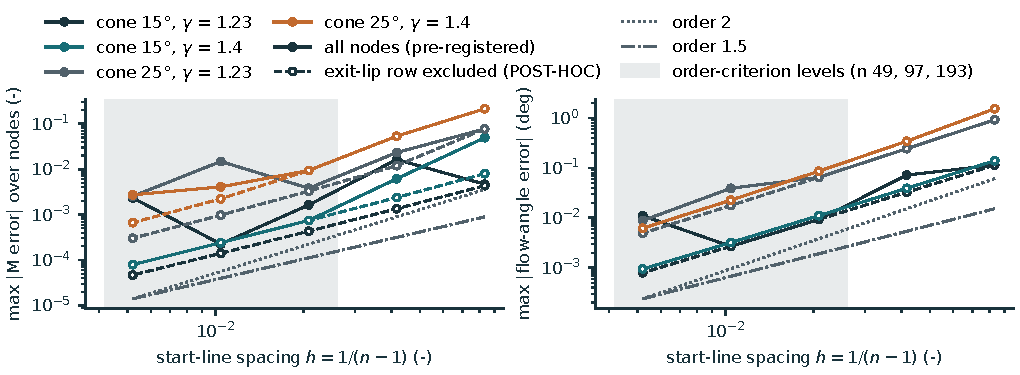
\includegraphics[width=\linewidth]{figures/e05_convergence_mach.pdf}
\caption{E05: production bounded net against exact source flow in cones. (a)~Maximum
Mach error over all nodes against start-line spacing $h$ for the four cone/$\gamma$
cases ($n=13$--193). Solid: all-node series, the pre-registered FAIL basis. Dashed
with open markers: the exit-lip row excluded (POST-HOC). Reference slopes of orders 2
and 1.5; grey band: criterion levels $n=49$, 97, 193. (b)~The same for the maximum
$\theta$ error (deg). Evidence class: verification. Recorded status: FAIL. Script:
\protect\code{scripts/moc_ext_e05_source_flow_oracle.py}.}
\label{fig:e05}
\end{figure}

\begin{figure}[htbp]
\centering
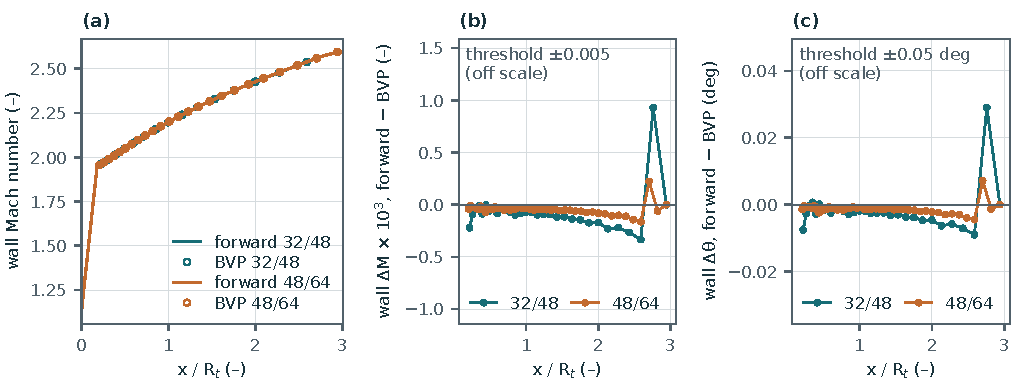
\includegraphics[width=\linewidth]{figures/e07b_exit_limited_replay.pdf}
\caption{E07b: exit-limited replay of the accepted Nozzle-B walls. (a)~Wall Mach
against $x/\Rt$: forward net (lines) and BVP wall nodes (circles), 32/48 and 48/64.
(b)~Wall $\Delta M\times10^3$ and (c)~wall $\Delta\theta$ (deg), forward minus BVP;
the diagnostic thresholds $\pm0.005$ and $\pm0.05^\circ$ are off scale. Evidence
class: verification (code-to-code; both algorithms share the KL start line). Recorded
status: PASS-DIAGNOSTIC. Script: \protect\code{scripts/moc_ext_e07b_exit_limited_replay.py}.}
\label{fig:e07b}
\end{figure}

\subsection{Transonic start line}\label{sec:exp-startline}
\textbf{E09, E09b, E09c} are discussed in Section~\ref{sec:kl} and shown in
Figs.~\ref{fig:e09} and~\ref{fig:e09c}. E09's replay part is INCOMPLETE, because no
variant reached the exit in the production net. E09c is a forward replay on the
KL-V0-optimised wall, not a corrected design, and D-K0-BVP is not approved (D10).

\begin{figure}[htbp]
\centering
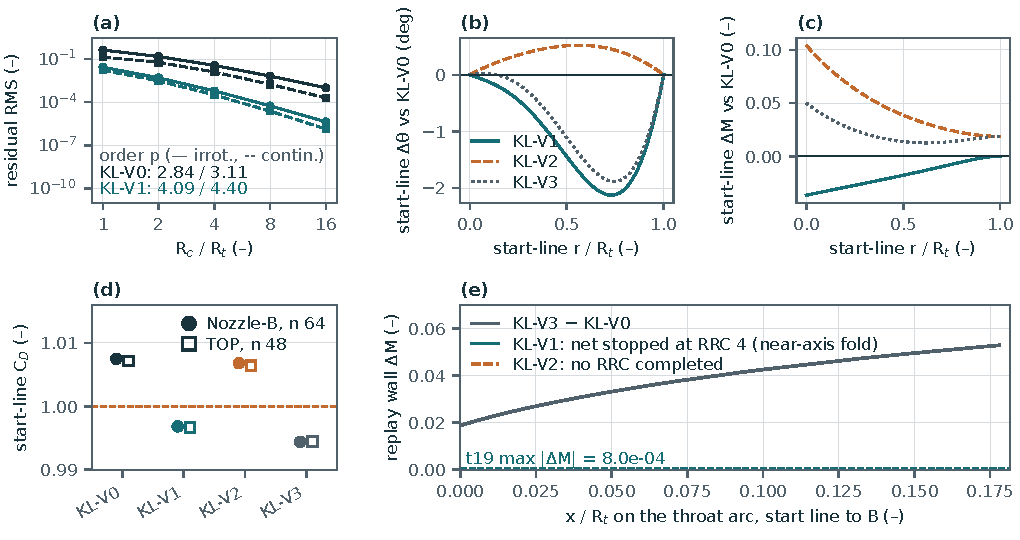
\includegraphics[width=\linewidth]{figures/e09_kl_variants.pdf}
\caption{E09: KL start-line variants (DIAGNOSTIC). (a)~Series-residual RMS against
$R_c/R_t$ at $\gamma=1.23$, for irrotationality and continuity; fitted orders 2.84/3.11
(KL-V0) and 4.09/4.40 (KL-V1). (b, c)~Start-line $\Delta\theta$ and $\Delta M$ relative
to KL-V0 against $r/\Rt$ for KL-V1 to KL-V3 (Nozzle-B, $R_u/R_t=1.5$, $n=64$).
(d)~$C_D$ by variant (Nozzle-B $n=64$; TOP $\gamma=1.2$, $n=48$). (e)~Forward-replay
wall $\Delta M$, KL-V3 minus KL-V0, along the throat arc to B on the 48/64 wall;
KL-V1 stopped at RRC~4 and KL-V2 completed no RRC; dashed: t19 maximum
$|\Delta M|=8.0\times10^{-4}$. Evidence class: verification (a); neither (b--e).
Recorded status: PASS-DIAGNOSTIC. Script: \protect\code{scripts/moc_ext_e09_kl_variants.py}.}
\label{fig:e09}
\end{figure}

\begin{figure}[htbp]
\centering
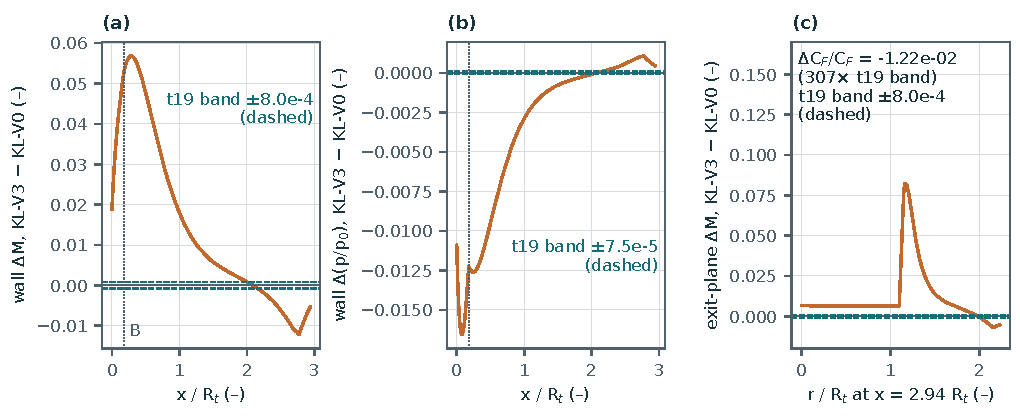
\includegraphics[width=\linewidth]{figures/e09c_k0b_replay.pdf}
\caption{E09c: KL-V3 replay of the accepted 48/64 Nozzle-B wall in the E07b harness.
(a)~Wall $\Delta M$, KL-V3 minus KL-V0, against $x/\Rt$, with B marked and the t19 band
$\pm8.0\times10^{-4}$. (b)~Wall $\Delta(p/p_0)$, band $\pm7.5\times10^{-5}$.
(c)~Exit-plane $\Delta M$ against $r/\Rt$ at $x=2.94\,\Rt$;
$\Delta C_F/C_F=-1.22\times10^{-2}$ (307 times the band). This is a forward replay on
the KL-V0-optimised wall, not a corrected design. Evidence class: neither
(diagnostic). Recorded status: PASS-DIAGNOSTIC. Script:
\protect\code{scripts/moc_ext_e09c_k0b_replay.py}.}
\label{fig:e09c}
\end{figure}

\subsection{Thermodynamics, geometry and separation}\label{sec:exp-thermo}\label{sec:exp-geometry}\label{sec:exp-separation}
E03's reference is the thermally perfect integral
\cite[Eqs.~4.35--4.36, PDF p.~186]{anderson}, \cite[Eq.~200, thermally perfect;
Eq.~199 general]{ames1953}. It passes the constant-$c_p$ limit, and the substitution
errors reject local-$\gamma$ use (Section~\ref{sec:g1}). E02, E02b and E04 are in
Section~\ref{sec:geometry-arch}. E08 and E08b are in Section~\ref{sec:g3}; they are
screening comparisons on an inviscid vacuum wall and say nothing about which criterion
is right.

\subsection{Shocks, viscous coupling and derivatives}\label{sec:exp-shocks}\label{sec:exp-viscous}\label{sec:exp-derivatives}
\textbf{E10 and E10b.} E10 is INCOMPLETE: the net stores no bell wall state, so H2 and
the envelope part of H3 were not evaluated (Fig.~\ref{fig:e10}). The straight-shock
bound $p_{02}/p_{01}=0.917$ cannot be tested, because no open numeric TOP
internal-shock data were found \cite[Sec.~3.5, PDF p.~26]{ostlund}, \cite{ruf2010}.

E10b accepted 136 bell wall nodes upstream of the first reversed cell. Neither their
straight $C^-$ nor the planar simple-wave envelope (Prandtl--Meyer relation
\cite[Eq.~4.44, PDF p.~187]{anderson}; envelope criterion
\cite[Secs.~24--25]{courant1944}) intersects inside the nozzle, so H2 is not supported.

\textbf{E11 and E11b} are FAIL-FEASIBILITY (Section~\ref{sec:g3}).

\textbf{E12, E12-diag-branch, E12b} (Fig.~\ref{fig:e12}). The Taylor test passes inside
event-free windows, but 36 ($J_1$) and 42 ($J_3$) jumps remain unexplained. In E12b,
the forward $J_1$ fit spans only one decade at all three points. The backward fit
passes (slope 1.988) at 27.2975$^\circ$ and 27.7975$^\circ$, but spans one decade at
28.2975$^\circ$.

\begin{figure}[htbp]
\centering
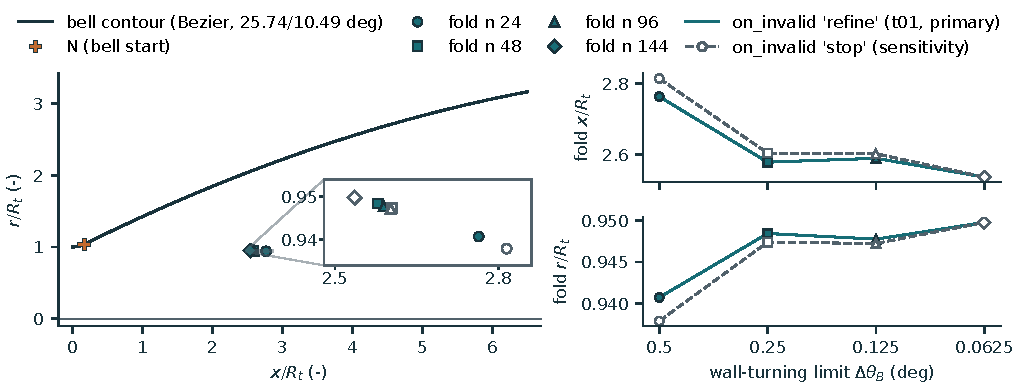
\includegraphics[width=\linewidth]{figures/e10_fold_envelope.pdf}
\caption{E10: fold on the current-chart TOP bell ($\Rt=20$\,mm, $\varepsilon=10$, 80\,\%,
$\gamma=1.2$). (a)~Bell contour (geometry from \protect\code{bell_nozzle_contour},
not a MOC run) with N and the four fold points of the primary
\protect\code{on_invalid='refine'} runs; the inset zooms on the fold cluster, with the
'stop' folds as open markers. (b)~Fold $x/\Rt$ and (c)~fold $r/\Rt$ against the
wall-turning limit (0.5 to $0.0625^\circ$, $n=24$ to 144); 'refine' solid, 'stop'
dashed. Evidence class: neither. Recorded status: INCOMPLETE. Script:
\protect\code{scripts/moc_ext_e10_top_fold_envelope.py}.}
\label{fig:e10}
\end{figure}

\begin{figure}[htbp]
\centering
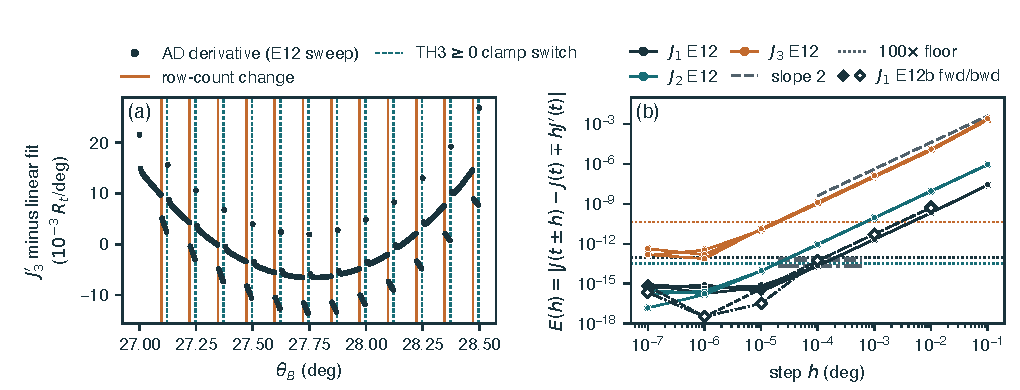
\includegraphics[width=\linewidth]{figures/e12_taylor_events.pdf}
\caption{E12: JAX throat kernel on the Nozzle-B arc. (a)~$\theta_B$ sweep 27.0--28.5$^\circ$
(301 points): $\dd J_3/\dd\theta_B$ minus its linear fit ($10^{-3}\,\Rt$/deg); solid
lines mark the 12 row-count changes and dashed lines the 12 TH3-clamp switches.
(b)~Taylor remainder $E(h)$ against $h$. Panel (b) mixes pre-registered E12 data
(solid: forward remainders of $J_1$, $J_2$, $J_3$ at 27.23, 27.73 and 28.23$^\circ$;
dotted: each output's 100$\times$ noise floor) with post-hoc E12b data ($J_1$ at
27.7975$^\circ$: forward dashed, backward dash-dot), distinguished by line style;
slope-2 reference. Evidence class: verification. Recorded status: E12 FAIL; E12b FAIL
(POST-HOC). Script: \protect\code{scripts/moc_ext_e12_jax_kernel_taylor.py}.}
\label{fig:e12}
\end{figure}

\subsection{CFD case writer and benchmark data}\label{sec:exp-cfd}\label{sec:exp-benchmark}
\textbf{E13} is a prototype pending D1; nothing about the flow is established until the
user runs the cases (Section~\ref{sec:cfd}).

\textbf{E14} is INFEASIBLE. Farley and Campbell's contours are 8/10 streamlines of
Clippinger's sharp-throat nozzles with boundary-layer corrections
\cite[PDF pp.~4, 19]{farley1960}. The forward net cannot regenerate the corrected walls
from published data without improvising the throat. Their wall pressures are plotted
only against $A/A_{cr}$ \cite[Fig.~10, PDF pp.~26--27]{farley1960}.

\section{Roadmap in dependency order}
\label{sec:roadmap}
Table~\ref{tab:roadmap} and Figure~\ref{fig:milestones} give the dependency order and
the user gates; deliverables and acceptance are in the gap sections. All milestones
except C0 and D0 are opt-in, and D0 needs a user decision.

\textbf{Changes from the draft.} Kept: C0, N0, N1, T0--T3, V0, V1, S1, A0 and D0.
Split: S0 and M0. Separated out: N2, S2 and V2. New: G0, Q0, X0, K0, B0, CFD0 and CFD1.

\begin{table}[htbp]
\centering\footnotesize
\caption{Milestones in dependency order, read down the left half and then the right
half. Gates are user decisions or source acquisitions (acq.).}
\label{tab:roadmap}
\begin{tabular}[t]{@{}lll@{}}
\toprule\textbf{ID} & \textbf{Depends on} & \textbf{Gate}\\\midrule
C0 & -- & --\\
G0 & C0 & D7, D11\\
Q0 & -- & --\\
X0 & -- & --\\
K0 & X0 & D3, D4, D10\\
B0 & -- & --\\
N0 & C0, X0 & --\\
N1 & N0, K0 & --\\
S0a & N0 & --\\
N2 & N1, S0a & --\\
T0 & C0 & --\\
T1 & N0, T0, K0 & --\\
T2 & T1 & acq.\ D2\\
\bottomrule
\end{tabular}\hspace{2.5em}
\begin{tabular}[t]{@{}lll@{}}
\toprule\textbf{ID} & \textbf{Depends on} & \textbf{Gate}\\\midrule
T3 & T2, N0, S0a & acq.\ D2\\
S0 & T0 & --\\
S1 & N0, S0, S0a, T0 & acq.\ D2\\
S2 & S1 & --\\
V0 & B0, N0, S0a, T0 & D9\\
V1 & N0, B0 & D5\\
V2 & V1, S1 & D6\\
CFD0 & C0, G0 & D1\\
CFD1 & CFD0, X0 & D1\\
M0 & C0, G0, N0, N1$^{\dagger}$ & D8, D10\\
A0 & X0, N0, B0, CFD1, M0 & --\\
D0 & A0, N1, M0 & user decision\\
\multicolumn{3}{@{}l}{\scriptsize $^{\dagger}$N1 applies to M0b only.}\\
\bottomrule
\end{tabular}
\end{table}

% Generated by builds/moc_extensions_plan_2026-11-21/writer_t/gen_milestones.py from
% builds/moc_extensions_plan_2026-11-21/opus_a/plan_record.json (transitive reduction of milestones[].depends_on).
% Do not edit by hand; checked by writer_t/check_milestone_edges.py.
\begin{figure}[htbp]
\centering
\begin{tikzpicture}[x=1in,y=1in,
  ms/.style={draw=teal,line width=0.5pt,fill=white,rounded corners=2pt,text=ink,
    font=\sffamily\fontsize{8}{8.6}\selectfont,align=center,inner xsep=3pt,inner ysep=1pt,
    text width=0.80in-6pt,minimum width=0.80in,minimum height=0.40in},
  gated/.style={ms,draw=accent,dash pattern=on 2pt off 1.2pt},
  dep/.style={draw=ink!80,line width=0.45pt,-{Stealth[length=1.5mm,width=1.1mm]}},
  band/.style={fill=pale,draw=none,rounded corners=3pt},
  lane/.style={font=\sffamily\scriptsize\bfseries,text=teal,align=left,anchor=west,
    text width=0.56in,inner sep=0pt}]
% lane bands
\fill[band] (0,0.000) rectangle (6.790,-0.470);
\node[lane] at (0.07,-0.235) {CFD};
\fill[band] (0,-0.600) rectangle (6.790,-1.070);
\node[lane] at (0.07,-0.835) {Integration};
\fill[band] (0,-1.130) rectangle (6.790,-2.070);
\node[lane] at (0.07,-1.600) {Infra-\\structure};
\fill[band] (0,-2.130) rectangle (6.790,-2.600);
\node[lane] at (0.07,-2.365) {Primal/AD};
\fill[band] (0,-2.660) rectangle (6.790,-3.130);
\node[lane] at (0.07,-2.895) {Thermo-\\dynamics};
\fill[band] (0,-3.240) rectangle (6.790,-4.180);
\node[lane] at (0.07,-3.710) {Viscous/\\separation};
\fill[band] (0,-4.240) rectangle (6.790,-5.180);
\node[lane] at (0.07,-4.710) {Shocks};
% milestones
\node[gated] (CFD0) at (3.180,-0.235) {\textbf{CFD0}\enspace{\tiny\color{accent}D1}\\OpenFOAM case writer};
\node[gated] (CFD1) at (4.250,-0.235) {\textbf{CFD1}\enspace{\tiny\color{accent}D1}\\Euler comparison};
\node[gated] (M0) at (4.250,-0.835) {\textbf{M0}\enspace{\tiny\color{accent}D8, D10}\\MOC$\to$MDO coupling};
\node[ms] (A0) at (5.320,-0.835) {\textbf{A0}\\Accuracy envelope};
\node[gated] (D0) at (6.390,-0.835) {\textbf{D0}\enspace{\tiny\color{accent}user decision}\\Default promotion};
\node[ms] (C0) at (1.040,-1.365) {\textbf{C0}\\Shared result contract};
\node[gated] (G0) at (2.110,-1.365) {\textbf{G0}\enspace{\tiny\color{accent}D7, D11}\\Length convention};
\node[ms] (Q0) at (6.390,-1.365) {\textbf{Q0}\\Diagnostic atlas};
\node[ms] (X0) at (1.040,-1.835) {\textbf{X0}\\Exact-solution oracles};
\node[gated] (K0) at (2.110,-1.835) {\textbf{K0}\enspace{\tiny\color{accent}D3, D4, D10}\\Transonic start line};
\node[ms] (B0) at (3.180,-1.835) {\textbf{B0}\\Benchmark data assets};
\node[ms] (N0) at (2.110,-2.365) {\textbf{N0}\\General-wall primal, tape};
\node[ms] (N1) at (3.180,-2.365) {\textbf{N1}\\Differentiable forward net};
\node[ms] (N2) at (6.390,-2.365) {\textbf{N2}\\Topology-event policy};
\node[ms] (T0) at (2.110,-2.895) {\textbf{T0}\\Thermo-state provider};
\node[ms] (T1) at (3.180,-2.895) {\textbf{T1}\\Thermally perfect MOC};
\node[gated] (T2) at (4.250,-2.895) {\textbf{T2}\enspace{\tiny\color{accent}acq.~D2}\\Equilibrium MOC};
\node[gated] (T3) at (6.390,-2.895) {\textbf{T3}\enspace{\tiny\color{accent}acq.~D2}\\Finite-rate MOC};
\node[gated] (V1) at (4.250,-3.475) {\textbf{V1}\enspace{\tiny\color{accent}D5}\\Separation onset};
\node[gated] (V0) at (5.320,-3.945) {\textbf{V0}\enspace{\tiny\color{accent}D9}\\Attached BL coupling};
\node[gated] (V2) at (6.390,-3.945) {\textbf{V2}\enspace{\tiny\color{accent}D6}\\RSS, side loads (scope)};
\node[ms] (S0a) at (3.929,-4.475) {\textbf{S0a}\\Envelope locator};
\node[ms] (S0) at (3.394,-4.945) {\textbf{S0}\\General-EOS jump operator};
\node[gated] (S1) at (4.892,-4.945) {\textbf{S1}\enspace{\tiny\color{accent}acq.~D2}\\Fitted internal shock};
\node[ms] (S2) at (6.390,-4.945) {\textbf{S2}\\Interactions (scope)};
% dependency edges: transitive reduction, one \draw[dep] per drawn edge (prerequisite -> dependent)
\draw[dep] (A0.east) -- (D0.west); % A0 -> D0
\draw[dep] ([yshift=0.075in]B0.east) .. controls (4.167,-1.760) and (4.139,-1.254) .. (4.705,-1.100) .. controls (4.705,-1.100) and (4.745,-1.100) .. (4.745,-1.100) .. controls (4.851,-1.053) and (4.804,-0.910) .. ([yshift=-0.075in]A0.west); % B0 -> A0
\draw[dep] (B0.east) .. controls (3.980,-1.835) and (4.033,-2.040) .. (4.428,-2.100) .. controls (4.428,-2.100) and (4.607,-2.100) .. (4.607,-2.100) .. controls (4.920,-2.363) and (4.607,-3.870) .. ([yshift=0.075in]V0.west); % B0 -> V0
\draw[dep] ([yshift=-0.075in]B0.east) .. controls (3.715,-1.910) and (3.580,-3.351) .. (3.715,-3.475) .. controls (3.715,-3.475) and (3.755,-3.475) .. (3.755,-3.475) .. controls (3.800,-3.484) and (3.804,-3.513) .. ([yshift=-0.037in]V1.west); % B0 -> V1
\draw[dep] (C0.east) -- (G0.west); % C0 -> G0
\draw[dep] ([yshift=-0.068in]C0.east) .. controls (1.575,-1.433) and (1.440,-2.248) .. (1.575,-2.365) .. controls (1.575,-2.365) and (1.615,-2.365) .. (1.615,-2.365) .. controls (1.660,-2.374) and (1.664,-2.403) .. ([yshift=-0.037in]N0.west); % C0 -> N0
\draw[dep] ([yshift=-0.135in]C0.east) .. controls (1.535,-1.500) and (1.440,-2.806) .. (1.535,-2.895) .. controls (1.535,-2.895) and (1.557,-2.895) .. (1.575,-2.895) .. controls (1.636,-2.895) and (1.649,-2.895) .. (T0.west); % C0 -> T0
\draw[dep] (CFD0.east) -- (CFD1.west); % CFD0 -> CFD1
\draw[dep] (CFD1.east) .. controls (4.916,-0.235) and (4.654,-0.760) .. ([yshift=0.075in]A0.west); % CFD1 -> A0
\draw[dep] ([yshift=0.037in]G0.east) .. controls (2.780,-1.327) and (2.510,-0.235) .. (CFD0.west); % G0 -> CFD0
\draw[dep] ([yshift=-0.037in]G0.east) .. controls (3.158,-1.403) and (3.202,-0.873) .. ([yshift=-0.037in]M0.west); % G0 -> M0
\draw[dep] ([yshift=0.037in]K0.east) .. controls (2.556,-1.797) and (2.579,-1.797) .. (2.605,-1.835) .. controls (2.605,-1.835) and (2.605,-2.100) .. (2.605,-2.100) .. controls (2.647,-2.208) and (2.664,-2.290) .. ([yshift=0.075in]N1.west); % K0 -> N1
\draw[dep] ([yshift=-0.037in]K0.east) .. controls (2.556,-1.873) and (2.560,-1.844) .. (2.605,-1.835) .. controls (2.605,-1.835) and (2.685,-1.835) .. (2.685,-1.835) .. controls (2.780,-1.921) and (2.685,-2.760) .. ([yshift=0.135in]T1.west); % K0 -> T1
\draw[dep] (M0.east) -- (A0.west); % M0 -> A0
\draw[dep] (N0.east) -- (N1.west); % N0 -> N1
\draw[dep] ([yshift=-0.135in]N0.east) .. controls (2.605,-2.500) and (2.510,-3.622) .. (2.605,-3.710) .. controls (2.605,-3.710) and (3.180,-3.710) .. (3.180,-3.710) .. controls (3.498,-3.915) and (3.180,-4.475) .. (S0a.west); % N0 -> S0a
\draw[dep] ([yshift=-0.045in]N0.east) .. controls (2.605,-2.410) and (2.547,-2.539) .. (2.605,-2.630) .. controls (2.669,-2.730) and (2.661,-2.828) .. ([yshift=0.068in]T1.west); % N0 -> T1
\draw[dep] ([yshift=-0.090in]N0.east) .. controls (2.600,-2.455) and (2.528,-2.584) .. (2.605,-2.630) .. controls (2.605,-2.630) and (3.755,-2.630) .. (3.755,-2.630) .. controls (3.850,-2.714) and (3.755,-3.438) .. ([yshift=0.037in]V1.west); % N0 -> V1
\draw[dep] ([yshift=0.075in]N1.east) .. controls (3.755,-2.290) and (3.716,-1.640) .. (3.755,-1.100) .. controls (3.755,-1.100) and (3.755,-0.835) .. (3.755,-0.835) .. controls (3.781,-0.798) and (3.804,-0.798) .. ([yshift=0.037in]M0.west); % N1 -> M0
\draw[dep] (N1.east) -- (N2.west); % N1 -> N2
\draw[dep] (S0.east) -- (S1.west); % S0 -> S1
\draw[dep] ([yshift=0.112in]S0a.east) .. controls (5.227,-4.363) and (4.543,-3.081) .. (5.320,-2.630) .. controls (5.320,-2.630) and (5.498,-2.630) .. (5.498,-2.630) .. controls (5.731,-2.587) and (5.753,-2.440) .. ([yshift=-0.075in]N2.west); % S0a -> N2
\draw[dep] ([yshift=-0.112in]S0a.east) .. controls (4.476,-4.588) and (4.345,-4.870) .. ([yshift=0.075in]S1.west); % S0a -> S1
\draw[dep] ([yshift=0.037in]S0a.east) .. controls (4.944,-4.438) and (5.064,-4.261) .. (5.677,-4.210) .. controls (5.677,-4.210) and (5.775,-4.210) .. (5.775,-4.210) .. controls (5.990,-4.029) and (5.775,-2.970) .. ([yshift=-0.075in]T3.west); % S0a -> T3
\draw[dep] ([yshift=-0.037in]S0a.east) .. controls (4.428,-4.513) and (4.329,-4.282) .. (4.428,-4.210) .. controls (4.428,-4.210) and (4.607,-4.210) .. (4.607,-4.210) .. controls (4.766,-4.166) and (4.755,-4.020) .. ([yshift=-0.075in]V0.west); % S0a -> V0
\draw[dep] (S1.east) -- (S2.west); % S1 -> S2
\draw[dep] ([yshift=0.075in]S1.east) .. controls (5.587,-4.870) and (5.535,-4.569) .. (5.815,-4.475) .. controls (5.815,-4.475) and (5.895,-4.475) .. (5.895,-4.475) .. controls (5.990,-4.397) and (5.895,-3.983) .. ([yshift=-0.037in]V2.west); % S1 -> V2
\draw[dep] ([yshift=-0.135in]T0.east) .. controls (2.823,-3.030) and (2.510,-4.679) .. (2.823,-4.945) .. controls (2.823,-4.945) and (2.917,-4.945) .. (S0.west); % T0 -> S0
\draw[dep] (T0.east) -- (T1.west); % T0 -> T1
\draw[dep] ([yshift=-0.068in]T0.east) .. controls (2.780,-2.963) and (2.587,-3.343) .. (2.823,-3.475) .. controls (2.823,-3.475) and (3.002,-3.475) .. (3.002,-3.475) .. controls (3.884,-3.582) and (4.031,-3.945) .. (V0.west); % T0 -> V0
\draw[dep] (T1.east) -- (T2.west); % T1 -> T2
\draw[dep] (T2.east) -- (T3.west); % T2 -> T3
\draw[dep] (V1.east) .. controls (5.167,-3.475) and (5.584,-3.475) .. (5.775,-3.710) .. controls (5.775,-3.710) and (5.775,-3.945) .. (5.775,-3.945) .. controls (5.820,-3.982) and (5.892,-3.908) .. ([yshift=0.037in]V2.west); % V1 -> V2
\draw[dep] ([yshift=0.075in]X0.east) .. controls (1.753,-1.760) and (1.440,-0.778) .. (1.753,-0.535) .. controls (1.753,-0.535) and (3.715,-0.535) .. (3.715,-0.535) .. controls (3.818,-0.477) and (3.732,-0.310) .. ([yshift=-0.075in]CFD1.west); % X0 -> CFD1
\draw[dep] (X0.east) -- (K0.west); % X0 -> K0
\draw[dep] ([yshift=-0.075in]X0.east) .. controls (1.526,-1.910) and (1.543,-1.788) .. (1.615,-1.835) .. controls (1.615,-1.835) and (1.615,-2.100) .. (1.615,-2.100) .. controls (1.637,-2.209) and (1.615,-2.328) .. ([yshift=0.037in]N0.west); % X0 -> N0
% legend
\node[ms,minimum width=0.30in,text width=0.24in,minimum height=0.15in,inner ysep=0pt] at (5.100,-0.135) {\textbf{X0}};
\node[font=\sffamily\scriptsize,text=ink,anchor=west,inner sep=1pt] at (5.280,-0.135) {milestone};
\draw[dep] (5.930,-0.135) -- (6.190,-0.135);
\node[font=\sffamily\scriptsize,text=ink,anchor=west,inner sep=1pt] at (6.210,-0.135) {depends on};
\node[gated,minimum width=0.30in,text width=0.24in,minimum height=0.15in,inner ysep=0pt] at (5.100,-0.345) {\textbf{G0}};
\node[font=\sffamily\scriptsize,text=ink,anchor=west,inner sep=1pt] at (5.280,-0.345) {gated: decision \textcolor{accent}{D$n$} or \textcolor{accent}{acq.}};
\end{tikzpicture}
\caption{Milestone dependency graph. Arrows run from prerequisite to dependent; edges implied by transitivity are omitted; the roadmap table lists all dependencies. Lanes group milestones by subject; position runs left to right in dependency order, with milestones that nothing depends on placed at the right. Q0 has no dependencies. Dashed orange outlines mark gates: a user decision (D1--D11) or a paywalled-source acquisition under D2. For K0 only the opt-in corrections K0b are gated; CFD1 also needs the user to run the cases.}
\label{fig:milestones}
\end{figure}


\keep{8}
\textbf{First package, in dependency order.}
\begin{enumerate}
\item C0, the result contract, which changes only result typing and refusals.
\item X0, the exact oracles, with the MOC-27 lip-row repair and the midpoint-limit test.
\item G0, after D7 and D11.
\item K0b, after D3 and D4, followed by the approval-gated re-solve (D10).
\item N0 and T0.
\item CFD0, once D1 is decided.
\end{enumerate}

\needspace{12\baselineskip}
\section{Acquisition list}
\label{sec:acquisitions}
None of these blocks the first package; acquiring any item is decision D2.
\begingroup\scriptsize\setlength{\tabcolsep}{5pt}
\par\addvspace{\LTpre}{\centering\begin{tabular}{@{}P{0.58\linewidth}P{0.17\linewidth}P{0.16\linewidth}@{}}
\toprule\textbf{Item} & \textbf{Status} & \textbf{Gates}\\\midrule
Zucrow--Hoffman Vol.~2 (exists \cite{clarke1978}); Broer 1958 full text \cite{broer1958}; Ferri 1954 \cite{ferri1954} & not held & T2, T3, S1, Young\\
Kliegel--Levine 1969 \cite{kliegel1969}; Hall 1962 \cite{hall1962} & paywalled; verdict done & K0 (optional)\\
Bartz 1955, 1965 \cite{bartz1955,bartz1965}; Elliott--Bartz--Silver \cite{elliott1963}, as cited in \cite{sp8120} & paywalled/unindexed & V0 alternative\\
Summerfield--Foster--Swan 1954 \cite{summerfield1954}, as cited in \cite{schmucker1984}; Kalt--Badal 1965 \cite{kalt1965}; Stark 2013 \cite{stark2013} & not held; paywalled & V1, D5\\
Crocco--Probstein (1964), Schilling (1962), as cited in \cite{sp8120,schmucker1984} & not held & V1 provenance\\
Clippinger, BRL Report 794 (1951), as cited in \cite{farley1960} & not held & B0 benchmark\\
Schomberg et al., AIAA 2014-3999, and Nguyen et al.\ 2003, as cited in \cite{schomberg2019} & not held & G0, D11 ($x_{mn}$)\\
Shock fitting: Salas 1976 \cite{salas1976}; Onofri--Paciorri 2017 \cite{onofri2017} & paywalled & S1\\
Benchmarks: \cite{hagemann2002,nasuti2009,verma2009,darwell1963,hoffman1987,dutton1981,hopkins1966}; Östlund--Bigert 1999 \cite{ostlund1999} & paywalled & S1, V2, K0, G3\\
Giles--Ulbrich Part~2 \cite{giles2010b} (Part~1 pointer from an unarchived copy \cite{giles2010a}); Giles--Pierce 2001 \cite{giles2001} & paywalled & G4 (S1)\\
Typeset copies \cite{lovely1999,celik2008}; Lovely thesis \cite{lovely2000} & identity only & CFD1\\
\bottomrule
\end{tabular}\par}\addvspace{\LTpost}
\endgroup

\section{Open decisions}
\label{sec:decisions}
These are the user's decisions; option (a) is recommended in each.

\textbf{D1, CFD reference} (lettered as in Section~\ref{sec:cfd}).
(a)~A write-only OpenFOAM v13 shockFluid writer (the E13 prototype); you run three
meshes on a Mac or Slurm cluster.
(b)~SU2.
(c)~An in-repo Euler solver.
(d)~No CFD for now.

\textbf{D2, Acquisitions.}
(a)~The gating items: Zucrow--Hoffman Vol.~2, Broer 1958 and Ferri 1954, plus
Clippinger 1951 if Farley--Campbell is wanted as a wall-pressure benchmark.
(b)~Also the boundary-layer, separation, shock-fitting and transonic items in
Section~\ref{sec:acquisitions}.
(c)~None, with the affected acceptance explicitly limited.

\textbf{D3, KL start line.} The sign error is confirmed. In a diagnostic forward replay
on the accepted wall, which was optimised with the uncorrected series, KL-V3 moves $C_F$
by $-1.22$\,\%. This is not a corrected design (Section~\ref{sec:kl}).
(a)~Add KL-V3 (corrected sign with $M^*\to M$) as an opt-in start-line method with
tests, keeping the production series as the default.
(b)~Report only.
(c)~Make the corrected series the default, which re-baselines every Rao and TOP result,
including the accepted t19 profile.

\textbf{D4, Normalisation ($M^*$ versus $M$).}
(a)~Include it only within KL-V3. Alone, as KL-V2, it gives $C_D=1.0068$ and an early
near-axis failure.
(b)~A separate opt-in flag.
(c)~Report only.

\textbf{D5, Separation criterion behind the MDO margin.}
(a)~Keep Schmucker at the Q1D exit state, the more conservative evaluation here. Add
its $M_i\le5$ flag and an opt-in wall-state variant, and report Schilling (0.582
against 0.583), Kalt--Badal, Summerfield and TP-1207 as cross-checks.
(b)~Switch to Schilling 0.583.
(c)~Switch to TP-1207.

\textbf{D6, RSS and side loads.}
(a)~Explicit exclusion with a typed ``unavailable'' result, plus a report-only Schmucker
$K_g$ estimate.
(b)~Exclude entirely.
(c)~Develop the capability, which needs S1, unsteady CFD and data.

\textbf{D7, Bell-length convention.}
(a)~An explicit convention parameter everywhere, with current defaults kept; you then
choose the project default.
(b)~Revert to the sharp-corner cone.
(c)~Switch every module to SP-125 now, which shifts the MDO geometry by about $0.04R_t$
at 80\,\% length.

\textbf{D8, MOC in the MDO.}
(a)~Keep the default; add M0a tables, then M0b after N1.
(b)~Aim for a default switch after A0.
(c)~Use MOC only after the solve.

\textbf{D9, Viscous coupling.}
(a)~Defer the method choice until the weak-coalescence policy exists, keeping the TDK
displaced wall (which completed at $s=1$) as the baseline.
(b)~Transpiration now, with a similar fold risk.
(c)~Wait for Bartz or Elliott--Bartz--Silver.

\keep{9}
\textbf{D10, Runs over about 30 minutes.} Only a re-solve shows how much of the E09c
change survives in a corrected design.
(a)~Approve one corrected-start-line Nozzle-B refinement pair after K0b is implemented
and tested. The estimate is about 25 minutes, by analogy with the accepted pair
(1{,}497.5\,s for both levels including a recomputed baseline); allow up to about
50 minutes if the corrected start line needs more optimiser iterations.
(b)~No long runs.
(c)~Additionally, a forward-net domain sweep for M0a (hours).
The re-solve has \emph{not} been run or approved.

\textbf{D11, LEA benchmark reference.}
(a)~Restate it from the source as $R_d=0.5R_t$ and $x_E-x_N=15.0r_t$, with the
definition flagged as inferred and the strict tolerance unchanged.
(b)~Keep the current reference, declared as sharp-corner, throat-to-exit and
$R_d=0.382$.
(c)~Make the LEA length check report-only.
The contour fit favours (a) only weakly (E02b).

\bibliographystyle{unsrtnat-short}
\needspace{8\baselineskip}
\section*{References}\addcontentsline{toc}{section}{References}
\renewcommand{\bibsection}{}
\begin{multicols}{3}
\bibliography{references}
\end{multicols}
\end{document}
